%%%%%%%%%%%%%%%%%%%%%%% file template.tex %%%%%%%%%%%%%%%%%%%%%%%%%
%
% This is a general template file for the LaTeX package SVJour3
% for Springer journals.          Springer Heidelberg 2010/09/16
%
% Copy it to a new file with a new name and use it as the basis
% for your article. Delete % signs as needed.
%
% This template includes a few options for different layouts and
% content for various journals. Please consult a previous issue of
% your journal as needed.
%
%%%%%%%%%%%%%%%%%%%%%%%%%%%%%%%%%%%%%%%%%%%%%%%%%%%%%%%%%%%%%%%%%%%
%
% First comes an example EPS file -- just ignore it and
% proceed on the \documentclass line
% your LaTeX will extract the file if required
\begin{filecontents*}{example.eps}
%!PS-Adobe-3.0 EPSF-3.0
%%BoundingBox: 19 19 221 221
%%CreationDate: Mon Sep 29 1997
%%Creator: programmed by hand (JK)
%%EndComments
gsave
newpath
  20 20 moveto
  20 220 lineto
  220 220 lineto
  220 20 lineto
closepath
2 setlinewidth
gsave
  .4 setgray fill
grestore
stroke
grestore
\end{filecontents*}
%
\RequirePackage{fix-cm}
%
% \documentclass{svjour3}                     % onecolumn (standard format)
% \documentclass[smallcondensed]{svjour3}     % onecolumn (ditto)
% \documentclass[smallextended]{svjour3}       % onecolumn (second format)
\documentclass[twocolumn]{svjour3}          % twocolumn
%
\smartqed  % flush right qed marks, e.g. at end of proof
%
\usepackage{graphicx}
%
% \usepackage{mathptmx}      % use Times fonts if available on your TeX system
%
% insert here the call for the packages your document requires
%\usepackage{latexsym}
% etc.
%
% please place your own definitions here and don't use \def but
% \newcommand{}{}
%
% Insert the name of "your journal" with
\journalname{Journal of Signal Processing and Systems}
%
\usepackage{color}
\usepackage{listings}
\usepackage{pgfplots}
\pgfplotsset{compat=1.8}
\usepgfplotslibrary{groupplots}
\usepackage{tikz}
\usetikzlibrary{patterns}
\usepackage{booktabs}
\newcommand{\subparagraph}{}
\usepackage{titlesec}
\usepackage{multirow}
\usepackage{url}
\usepackage{amsmath}
% \usepackage{amsthm}
\usepackage{amsfonts}
\usepackage{subfig}
\usepackage{graphicx}
\usepackage{epstopdf}
\usepackage{paralist}
\usepackage[boxed,linesnumberedhidden]{algorithm2e}
\pagestyle{empty}
% \newtheorem{theorem}{Theorem}[section]
% \newtheorem{lemma}[theorem]{Lemma}
% \newtheorem{proposition}[theorem]{Proposition}
% \newtheorem{corollary}[theorem]{Corollary}
\usepackage{mdwlist}
\linespread{0.994}
% \usepackage{bibspacing}
\usepackage{color}
%\usepackage{hyperref}
\makeatletter
\newbox\sf@box
\newenvironment{SubFloat}[2][]%
{\def\sf@one{#1}%
\def\sf@two{#2}%
\setbox\sf@box\hbox
\bgroup}%
{ \egroup
\ifx\@empty\sf@two\@empty\relax
\def\sf@two{\@empty}
\fi
\ifx\@empty\sf@one\@empty\relax
\subfloat[\sf@two]{\box\sf@box}%
\else
\subfloat[\sf@one][\sf@two]{\box\sf@box}%
\fi}
\makeatother

\titlespacing*{\section}{0pt}{0.5cm}{0.3cm}
\titlespacing*{\subsection}{0pt}{0.5cm}{0.3cm}


\begin{document}

\title{Times square -- marriage of real-time and logical-time in GALS
  and synchronous languages%\thanks{Grants or other notes
%about the article that should go on the front page should be
%placed here. General acknowledgments should be placed at the end of the article.}
}
% \subtitle{Do you have a subtitle?\\ If so, write it here}

%\titlerunning{Short form of title}        % if too long for running head

\author{Heejong Park \and
        Zhenmin Li \and 
        Avinash Malik \and 
        Zoran Salcic % etc.
}

%\authorrunning{Short form of author list} % if too long for running head

\institute{H. Park \and Z. Li \and A. Malik \and Z. Salcic \at
  Department of Electrical and Computer Engineering\\
  38 Princes Street \\
  University of Auckland \\
  Auckland 1010 \\
  New Zealand \\
  % Tel.: +123-45-678910\\
  % Fax: +123-45-678910\\
  \email{hpar081@aucklanduni.ac.nz}           %  \\
}

\date{Received: date / Accepted: date}
% The correct dates will be entered by the editor


\maketitle

\newcommand{\hj}[1]{\textcolor{black}{#1}}
\begin{abstract}

	In this paper we introduce exact and non-exact real-time waits in the
	reactive Globally Asynchronous Locally Synchronous (GALS) programming
	languages and synchronous languages as their subset. The language
	constructs that allow use of real-time waits are illustrated on the
	SystemJ GALS language. They allow system designers to explicitly use,
	at the specification level, not only logical time but also real-time
	in order to control \hj{program execution}. We transform the real-time
	constructs into a logical model of time, and statically bound the
	amount of delay introduced by these constructs. In addition, the
	introduced concepts utilize execution platforms that allow finding
	best and worst reaction time of a GALS or synchronous program.


  \keywords{GALS languages \and Synchronous languages \and exact and non-exact delays}

\end{abstract}

\lstdefinestyle{sysj}{
  belowcaptionskip=1\baselineskip,
  breaklines=true,
  xleftmargin=\parindent,
  language=Java,
  showstringspaces=false,
  basicstyle=\scriptsize\ttfamily,
  keywordstyle=\bfseries\color{green!40!black},
  commentstyle=\itshape\color{purple!40!black},
  identifierstyle=\color{blue},
  stringstyle=\color{orange},
}

% \section{Introduction}
% \label{intro}
% Your text comes here. Separate text sections with
% \section{Section title}
% \label{sec:1}
% Text with citations \cite{RefB} and \cite{RefJ}.
% \subsection{Subsection title}
% \label{sec:2}
% as required. Don't forget to give each section
% and subsection a unique label (see Sect.~\ref{sec:1}).
% \paragraph{Paragraph headings} Use paragraph headings as needed.
% \begin{equation}
% a^2+b^2=c^2
% \end{equation}

% % For one-column wide figures use
% \begin{figure}
% % Use the relevant command to insert your figure file.
% % For example, with the graphicx package use
%   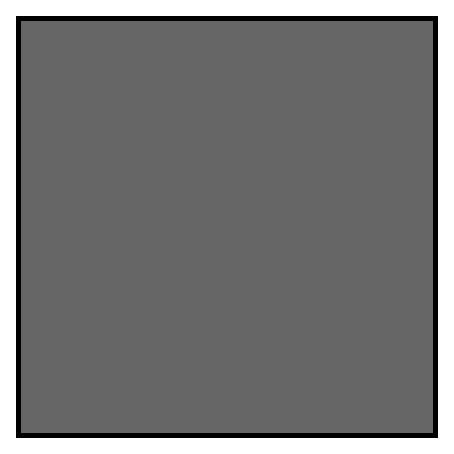
\includegraphics{example.eps}
% % figure caption is below the figure
% \caption{Please write your figure caption here}
% \label{fig:1}       % Give a unique label
% \end{figure}
% %
% % For two-column wide figures use
% \begin{figure*}
% % Use the relevant command to insert your figure file.
% % For example, with the graphicx package use
%   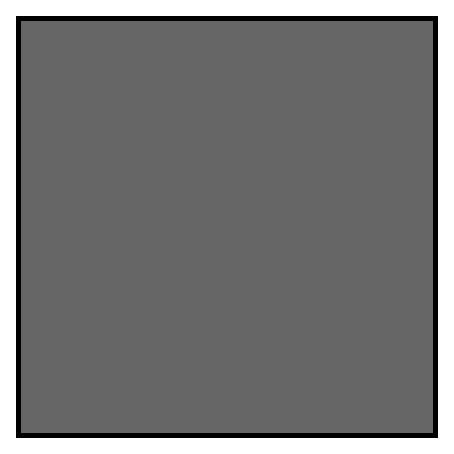
\includegraphics[width=0.75\textwidth]{example.eps}
% % figure caption is below the figure
% \caption{Please write your figure caption here}
% \label{fig:2}       % Give a unique label
% \end{figure*}
% %
% % For tables use
% \begin{table}
% % table caption is above the table
% \caption{Please write your table caption here}
% \label{tab:1}       % Give a unique label
% % For LaTeX tables use
% \begin{tabular}{lll}
% \hline\noalign{\smallskip}
% first & second & third  \\
% \noalign{\smallskip}\hline\noalign{\smallskip}
% number & number & number \\
% number & number & number \\
% \noalign{\smallskip}\hline
% \end{tabular}
% \end{table}


%\begin{acknowledgements}
%If you'd like to thank anyone, place your comments here
%and remove the percent signs.
%\end{acknowledgements}

% BibTeX users please use one of
%\bibliographystyle{spbasic}      % basic style, author-year citations
%\bibliographystyle{spmpsci}      % mathematics and physical sciences
%\bibliographystyle{spphys}       % APS-like style for physics
%\bibliography{}   % name your BibTeX data base

\section{Introduction and motivation}
\label{sec:intr-motiv}

Reactive languages~\cite{gber931,amal10} are a class of programming
languages used for designing and implementing reactive systems, which
continuously respond to input from their environment. These languages
have been successfully used in programming a plethora of systems such as
fly-by-wire in Airbus~\cite{eairbus}, security surveillance
systems~\cite{amal121}, etc. Usually these systems also need to meet
real-time constraints imposed by the environment. Yet, these languages
do not support describing real-time statements as first class language
constructs.  For example, one cannot describe a simple real-time delay
(postponement) of an operation for 0.2 ms. These languages are based on
formal semantics, essential for correct by construction code generation
and formally verifying functional properties of developed programs, but
leave nonfunctional properties such as timing behavior as an
implementation detail~\cite{boldt07}. Arguably, rightly so, because
physical time cannot be incorporated without information about the
underlying execution platform.  But, one can still reason in terms of
logical time. These languages support discrete logical clock rather than
a discrete physical (real-time) clock. The real-time period of the
discrete logical clock (also referred to as a logical tick) is not fixed
and it is determined by the speed of computation of the program for
different input signals. Unlike a discrete physical clock, which has
fixed real-time period, the period of the logical clock is elastic.
Although the timing model with logical clock has worked well for
reactive synchronous/GALS languages in designing discrete systems, there
is a need to introduce real-time since often, implementation models are
in the continuous or discrete real-time
domain~\cite{DBLP:journals/pieee/SifakisTY03}. This paper targets
enhancing the expressiveness of formal GALS and synchronous languages by
adding real-time constructs. These real-time constructs speed up the
design process by allowing system designers to explicitly program
real-time control logic within the language itself without relying on
external resources such as timers. Introduction of real-time as a
language construct allows verification of temporal properties of
programs before deployment.

%Moreover, adding timing
%capabilities as first class language constructs create additional
%opportunity for formally verifying functional and non-functional
%requirements before system deployment.

\subsection{Motivation via examples of real-time systems programmed in a
reactive language SystemJ}
\label{sec:motivating-example}

% system{
%  interface{
%   input signal TOUCH;
%   output signal GREEN_LIGHT;
%   output char channel S;
%   input char channel R;
%  }

Real-time operating systems~\cite{barry2009using} usually provide two
types of mechanisms for introducing real-time in the developed program:
(1) the ability to perform a timeout and (2) the ability to run tasks
periodically with some real-time period $T$. These mechanisms are
essential in many real-time applications for ensuring the correctness of
the program's behaviors. For example, an alarm controller for a retail
store may be required to wait for a specific amount of time, allowing an
owner to enter a password, before it triggers an alarm sound. In a
safety-critical applications, such as an artificial cardiac pacemaker
\cite{Singh:2012:CPC:2388936.2388948}, such real-time features are
indispensable; a pacemaker must be able to correctly monitor time
intervals between the heart's native electrical pulse in order to
control abnormal heart rhythms. Nevertheless, lack of real-time
constructs in the reactive languages \cite{gber931,amal10} makes them
difficult to be used in many real-time applications.

In order to close this gap, we would like to provide similar mechanisms
in reactive languages for real-time program development. In fact, we
provide \textit{exact} and \textit{non exact} real-time control
mechanisms -- a generalization of the two real-time mechanisms
introduced in real-time operating systems. In this section, a program
written in a reactive language called SystemJ is used as a motivating
example to illustrate the usefulness of such real-time control
statements.

\subsubsection{Programming using the non exact real-time control
  construct; the \textrm{\texttt{wait\_inbetween}} statement}
\label{sec:progr-using-non}

\begin{figure}[t!]
	\vspace{-10pt}
        \begin{SubFloat}{\label{delay:a}A human responsiveness
            system (HRTCS)}
        \begin{lstlisting}[style=sysj,morekeywords={sustain,send,receive,abort,await,emit,present,trap,pause,exit,wait_inbetween,wait_exact,suspend}]
{ // Clock-domain 1
while(true) {
  trap(T){
   // Abort if user touches the screen
   abort(TOUCH){
    {sustain GREEN_LIGHT;} //reaction R1
    || // synchronous parallel operator
    {
     //exit after any where from 50.3 to 200.3 ms.
     wait_inbetween(50.3 .. 200.3 ms); 
     exit(T); 
    } // reaction R2
   } do {send S(1);} // Send 1 if touched 
  } do {send S(0);} // Else Send 0
  pause; pause; pause; // pass some time before restarting
 }
}
>< // asynchronous operator
{ // Clock-domain 2
  while(true){ receive S; 
      if(#S == 1) counter++; else counter--;}
}
\end{lstlisting}
\end{SubFloat}
\begin{SubFloat}{\label{d:b}Timing diagram -- the X-axis shows the
    execution of the \texttt{wait\_inbetween} statement. The Y-axis is
    the time elapsed. The arrow shows one example of the expiration of
    the \mbox{\texttt{wait\_inbetween(50.3..200.3 ms)}} statement.}
  % \begin{figure}[h!]
    \centering
    \includegraphics[scale=0.7]{FF1}
  % \end{figure}
\end{SubFloat}
\caption{Programming a human responsiveness system (HRTCS) with
  \texttt{wait\_inbetween}}
% }
% \end{center}
\label{fig:1}
\end{figure}

The \texttt{wait\_inbetween(M..N)} statement postpones the program
control flow from proceeding to the following statement for a minimum of
$M$ time units and a maximum of $N$ time units, as shown in
Figure~\ref{d:b}.

Consider a machine used to test human response time and collect this
data for future research purposes. The machine switches on a green light
on a touch screen for anywhere \textit{in between} 50.3 ms to 200.3 ms,
if the user can touch this green light then she is successful and \hj{an
  integer \texttt{1} is sent to another process in order to increase an
  integer counter, if unsuccessful a \texttt{0} is sent instead to
  decrease the counter}. Different statistics and analyses on human
responsiveness can be based on the collected data.

The SystemJ pseudo-code~\cite{amal10} for such a system, along with the
expected timing behavior of the \texttt{wait\-\_inbetween} statement, is
shown in Figure~\ref{delay:a}. We use the SystemJ language in this
paper, because being a \textit{Globally Asynchronous Locally
Synchronous} (GALS) language it helps us easily describe a larger class
of systems (like HRTCS in Figure~\ref{delay:a}) compared to purely
synchronous languages like Esterel \cite{gber931}. Moreover, being a
super-set of Esterel, SystemJ allows us to explore the marriage of
real-time and logical time not only in the GALS, but also in the
synchronous setting.

The SystemJ program in Figure~\ref{delay:a} is divided into two
\hj{mutually asynchronous} clock-domains, the first clock-domain
continuously displays a green light (\texttt{GREEN\_LIGHT} signal) on
the touch screen sensor and waits for the user to respond. If the user
is able to touch the screen within the specified time of at least 50.3
ms and at most 200.3 ms, a positive response is sent to the second
clock-domain. All the SystemJ programming constructs used to implement
this system are described in Table~\ref{tab:1} \hj{and more details can
  be found in~\cite{amal10}}. The \texttt{wait\_inbetween}
specification, which models the non exact postponement between 50.3 ms
and 200.3 ms is not supported in the current language and cannot be
compiled with the current SystemJ compiler. We introduce such
\texttt{wait\_inbetween} statements in SystemJ. Such non exact real-time
mechanisms are useful for developing systems where the real-time
postponement is not known or should not be known a priori.

\subsubsection{Programming a timeout using the non exact real-time
  construct; the \texttt{wait\_atleast} statement}
\label{sec:progr-time-using}

\begin{figure}[b!]
	\centering
	\vspace{-10pt}
        \begin{SubFloat}{\label{dd:a}Timeout waiting for the input
            signal \texttt{DoorOpened}}
        \begin{lstlisting}[style=sysj,morekeywords={abort,await,emit,present,trap,pause,exit,wait_atleast,suspend}]
trap(T){
  abort(DoorOpened){
    wait_atleast(10000 ms);
    exit(T);  
  }
}
\end{lstlisting}
\end{SubFloat}
\begin{SubFloat}{\label{dd:b}Timing diagram -- the X-axis shows the
    execution of the \texttt{wait\_atleast} statement. The Y-axis is the
    time elapsed. The arrow shows one possible expiration of
    \texttt{wait\_atleast(10000 ms)} statement.}
\includegraphics[scale=0.7]{FF2}
\end{SubFloat}
\caption{Programming a timeout with \texttt{wait\_atleast}}
\label{dd}
\end{figure}

The \texttt{wait\_atleast(M)} statement is used to postpone the program
control flow from proceeding to the next statment for a minimum of $M$
time units. The maximum postponement is unbounded, but countable
(Figure~\ref{dd:b}).

There are many instances when one would like to wait on an input from
environment for only a specified amount of time. If the signal is not
received, then a timeout is generated so that the program can make
progress. Such a timeout programmed in the SystemJ pseudo-code along
with its timing behavior is shown in Figure~\ref{dd:a}. A part of the
SystemJ door alarm system is waiting on an input signal,
\texttt{DoorOpened}, from the environment for 10 seconds and makes
progress irrespective of the reception of this signal after 10 seconds.

The timing diagram, Figure~\ref{dd:b}, shows that the
\texttt{wait\-\_atleast} statement waits for a \textit{at least} 10
seconds, but unlike \texttt{wait\_inbetween} there is no upper bound.
For example in Figure~\ref{dd:b} program might proceed to the next
statement at anytime greater than or equal to 10 seconds (say 11
seconds) according to the semantics of \texttt{wait\_atleast}
statement. The statement following the \texttt{wait\_atleast} statement
is executed after a finite countable, but unbounded postponement. Such a
statement is useful for programming low priority tasks.


\subsubsection{Programming periodic tasks using the exact real-time
  construct; the \texttt{wait\_exact} statement}
\label{sec:progr-using-exact}

The previous wait statements are non exact, i.e., the \hj{time of}
execution of the statement following the wait statement cannot be
controlled exactly. The final variant we introduce allows doing exactly
that. We call it \texttt{wait\_exact(M)} and this statement can be used to
program exact timeouts, periodic tasks, etc.

\begin{figure}[t!]
  \centering
	\vspace{-10pt}
        \begin{SubFloat}{\label{pp:aa}Periodically emitting signal S}
        \begin{lstlisting}[style=sysj,morekeywords={emit,trap,pause,exit,wait_exact}]
while(true) { 
 wait_exact (1 ms); 
 emit S; 
 //do something 
}
\end{lstlisting}
\end{SubFloat}

\begin{SubFloat}{\label{p1:b}Timing diagram -- the X-axis shows the
    execution of the \texttt{wait\_exact} statement. The Y-axis is the
    time elapsed. The arrow shows the \textit{only} possible expiration
    of the \texttt{wait\_exact(1 ms)} statement.}
  \includegraphics[scale=0.7]{FF3}
\end{SubFloat}
  \caption{Programming a periodic task with wait\_exact}
  \label{fig:p1}
  \vspace{-10pt}
\end{figure}

One such example; periodic emission of a signal to the environment is
shown in Figure~\ref{pp:aa}. As before, upon execution of
\texttt{wait\_exact(1 ms)} statement, the time starts elapsing. But,
unlike in previous cases the following statement needs to be executed
exactly after 1 ms has passed, as shown in Figure~\ref{p1:b}.


%  LocalWords:  statment

%%% Local Variables: 
%%% mode: latex
%%% TeX-master: "template"
%%% End: 


The major motivations for introducing these real-time \textit{wait}
mechanisms and at the same time \textbf{contributions} of the paper are:
\hj{(1) real-time wait does not affect the model of logical time in
	SystemJ program as long as the amount of delay is within boundaries
that can be determined statically by program analysis.} (2) the waiting
model relies on the use of relative instead of absolute real-time, i.e.,
a wait in selected time units is counted from the beginning of the wait
statement and (3) these waiting mechanisms allow mixing behaviors with
real-time features and others with only logical time. All these as well
as semantics of the wait constructs are discussed and illustrated in the
rest of the paper. Our contributions can be further refined as follows:

\begin{enumerate*}
\item Real-time is specified in the $\mathbb{Q}^{>0}$ domain of numbers,
  i.e., non-negative rational numbers.
% \item We consider the property of \textit{non
%     maximal-parallelism}. \textit{Non-maximal parallelism:} There are
%   not always sufficient resources for processes to execute, so
%   effectively processes are allocated and scheduled with different
%   optimization criteria -- reducing computation time, reducing power
%   consumption, etc. This allocation and scheduling is an integral part
%   of any language compilation and needs to be considered when
%   introducing real-time waits.
\item We are the first, to our knowledge, to allow specification of
  both; exact and non-exact real-time in GALS and synchronous programs.
\item We shed light upon a key insight relating real-time and
  logical-time -- \textit{the resolution of any real-time statement is
    dependent on the worst case logical tick time} -- an aspect that
  seems to have escaped in the current literature on incorporating
  real-time in synchronous/GALS languages.
\end{enumerate*}

All aforementioned contributions require a single \textbf{assumption}
that real-time analyzable platforms are available that allow computing
the timing bounds of SystemJ programs. This assumption is necessary for
all hard real-time system implementations~\cite{wilhelm08}.

The rest of the paper is arranged as follows:
Section~\ref{sec:background} gives the background on SystemJ and related
techniques required for the rest of the paper.
Section~\ref{sec:intr-real-time} introduces real-time mechanisms in the
GALS paradigm and describes their compilation into logical time.
Section~\ref{sec:proof-correctness} sketches the correctness proofs for
the introduced algorithms. Section~\ref{sec:experimental-results} gives
the experimental results for a set of real-time applications. In
Section~\ref{sec:disc-perc-limit} we discuss the advantages and
limitations of the proposed approach. Section~\ref{sec:related-work}
positions this work in relation to other approaches to introducing
real-time in other languages. Finally, we conclude in
Section~\ref{sec:concl-future-work}.



%%% Local Variables: 
%%% mode: latex
%%% TeX-master: "template"
%%% End: 

\section{Background}
\label{sec:background}

\subsection{Brief introduction to SystemJ syntax, semantics and model of
  computation}
\label{sec:brief-intr-syst}

\begin{table}[tb]
\centering
\begin{minipage}{0.45\textwidth}
\caption{SystemJ kernel statements and their meaning}
  \begin{scriptsize}
   \begin{tabular}{|c|p{80pt}|}
     \hline                                                                                     
     \textbf{Kernel Statements} & \textbf{Meaning}\\                                            
     \hline                                                                                     
     \hline                                                                                     
     [\textbf{\texttt{input}}] [\textbf{\texttt{output}}]
     [\textbf{\texttt{type}}] \textbf{\texttt{signal}} S & declare signal S\\                                      
     \hline                                                                                     
     \textbf{\texttt{emit}} S [(value)] & broadcast signal S\\                                                    
     \hline                                                                                     
     \textbf{\texttt{present}} (S) \{p\} else \{q\}& do p if S is present, else do q\\                            
     \hline                                                                                     
     \textbf{\texttt{abort}} (S) \{p\} & preempt program p if S is present\\                                      
     \hline                                                                                     
     \textbf{\texttt{suspend}} (S)\{p\} & suspend p if S is present\\                                             
     \hline                                                                                     
     \textbf{\texttt{trap}} (T)\{p\ldots \textbf{\texttt{exit}} T\ldots\} & preempt p if exit is executed\\                         
     \hline                                                                                     
     p\textbf{\texttt{$||$}}q & run p and q in lock-step\\                                                        
     \hline                                                                                     
     p$><$q & run p and q asynchronously\\                                                      
     \hline                                                                                     
     \textbf{\texttt{send}} C([value]) & send a value through C, blocking
     send\\                                                 
     \hline                                                                                     
     \textbf{\texttt{receive}} C() & receive a value through C, blocking
     receive\\
     \hline                                                                                     
     \textbf{\texttt{pause}} & finish a tick and communicate
     with environment\\
     \hline                                                                                     
   \end{tabular}
 \label{tab:1}
  \end{scriptsize}
   % \footnotetext[1]{\scriptsize Uppercase}
 \end{minipage}
\end{table}

Table~\ref{tab:1} presents the SystemJ kernel statements used to program
the control flow. The data flow is programmed in the safe subset of
Java~\cite{scj2013} amenable to formal verification and timing analysis,
while avoiding all the pitfalls of programming in `C' style languages. A
number of derived statements also exist (e.g., \texttt{sustain},
\texttt{await}, etc.) that make programming reactive systems easier. The
\textit{Model of Computation} (MoC) of a simple SystemJ program is shown
in Figure~\ref{fig:2}.

SystemJ consists of entities called \textit{Clock Domains} (CDs), each
running at their individual pace, interacting with the environment via
signals and with each other using CSP~\cite{choa85} style rendezvous via
channels. Therefore, unlike other approaches that use broadcasting
signals as a communication method between asynchronous processes (e.g.
Multiclock-Esterel \cite{multiesterel}), SystemJ's channel provides a
safer way to exchange messages between clock-domains. Each CD has its
own notion of logical time. CDs are composed of one or more units called
reactions.  These reactions themselves can be composed of child
reactions forming a hierarchy. Each CD adheres to the \textit{perfect
synchrony} hypothesis, i.e., all statements execute instantaneously in
zero time. Only the \texttt{pause} statement consumes time, just like in
Esterel~\cite{gber931}. Consider the SystemJ program in
Figure~\ref{fig:2a}, it is waiting for an input signal producing logical
ticks (see Figure~\ref{fig:2c}). Once \texttt{A} is received at tick 1
or 4, output \texttt{O} is emitted to the environment instantaneously.

\subsection{Mapping logical time to physical time}
\label{sec:mapping-logical-time}

\begin{figure}[t!]
\centering
\begin{SubFloat}{\label{fig:2a}Simple SystemJ program}%...verbatim subfigure
	\hspace{1cm}
\begin{minipage}[b]{0.8\linewidth}% a minipage to control the width...
		\begin{lstlisting}[style=sysj,morekeywords={abort,await,emit,present,trap,pause,exit,delay,suspend}]
{
int counter = 0;
while(true){
 abort(immediate A){
  while(true) pause; 
 } // abort end
  emit O;
  if(counter != 0) 
  {/* java computation leading to WCRT */}
  ++counter;
 } // loop end
} // SystemJ CD end
\end{lstlisting}%
\end{minipage}%
\end{SubFloat}
%\hspace{1.5cm}%
% \begin{SubFloat}[Black box]{\label{fig:2b}Logical time in SystemJ}%
% \includegraphics[scale=0.4]{moc}
% \end{SubFloat}%
% \vspace{-10pt}

\begin{SubFloat}{\label{fig:2c}Mapping to physical time}%
% \includegraphics[scale=0.4]{phy.pdf_t}
\scalebox{0.68}{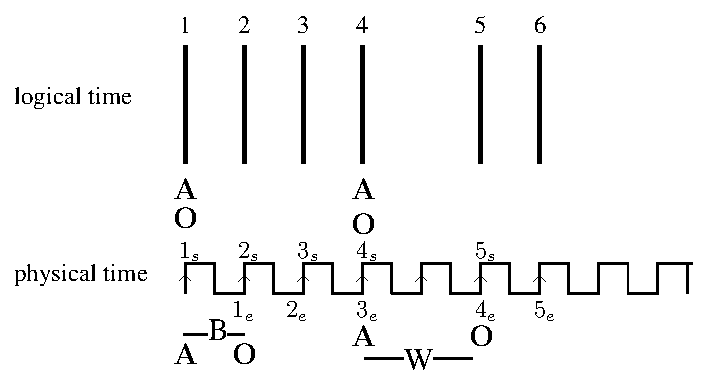
\includegraphics{phy_t.pdf}}
\end{SubFloat}%
\caption{Simple SystemJ example and corresponding MoC}
\label{fig:2}
\end{figure}

The perfect synchrony hypothesis is ideal for programming the
synchronous subset of SystemJ. Nevertheless, execution of every
statement requires $\delta$ physical time. Time for a logical tick can
thus be summarized as $\Delta = \mathcal{F} (\delta)$, where
$\mathcal{F}$ is the schedule. We call $\Delta$ the reaction
time. Depending upon the amount of computation required and the
schedule, $\Delta$ can vary. In order to satisfy the implicit
restriction imposed by the synchrony hypothesis -- no input event
\textit{from the environment} can be missed -- one needs to calculate
the \textit{Worst Case Reaction Time} (WCRT) and the resultant WCRT
needs to be smaller than the time between any two consecutive events on
any input, else the synchrony hypothesis is violated. Our static
analysis techniques to calculate the WCRT of a synchronous program is
presented in Section~\ref{sec:stat-analys-comp-1}. The opposite of the
WCRT, the shortest time for a reaction, is called the \textit{Best Case
  Reaction Time} (BCRT). Formally, let $\{\Delta_1, \Delta_2,\ldots,
\Delta_N\}$, be the set of all possible reaction times for some
CD. Then, $\exists i \in N, \mathrm{where\ } WCRT= max (\Delta_i)$,
similarly, $\exists j \in N$, where $BCRT = min (\Delta_j)$.


We denote the WCRT and BCRT in Figure~\ref{fig:2c} using \texttt{W} and
\texttt{B}, respectively. It shows a continuously running physical clock
(analogous to a clock in digital hardware), the numerical annotations on
the rising edge of the clock mark the logical ticks from
Figure~\ref{fig:2c}. The subscripts \texttt{s} and \texttt{e} for the
numbers show the start and end of the logical ticks, respectively. The
end of a logical tick and the start of the next logical tick happen
together. The figure also shows the mapping of the logical time to the
physical time. For example, the logical tick \texttt{1} starts at the
first rising edge and completes at the second rising edge of the
physical clock, whereas logical tick \texttt{4} starts at the $4^{th}$
rising edge, but finishes at the $6^{th}$ rising edge of the physical
clock. This difference can be accounted for by the Java computations
required when signal \texttt{A} is input by the environment (see
Figure~\ref{fig:2a}). This elasticity is inherent (and elegant) to both
Esterel and SystemJ.

% We now present a lemma with proof sketch (due to lack of space) that we
% require for the rest of the paper and is special to SystemJ, being a
% GALS language.

% \begin{lemma}
%   WCRT and BCRT analysis are invariant to values of conditional
%   expressions.
% \end{lemma}

% \begin{proof}
%   The physical time ($\delta$) taken by a conditional expression is at
%   best affected by the type rather than the value of the
%   conditional. Example, comparing the value of 2 floats might take
%   longer than comparing the value of 2 integer types on some given
%   platform. But, the time taken by the comparison instruction is
%   invariant to the value itself.
% \end{proof}

% \begin{lemma}
%   WCRT and BCRT analysis are invariant to channel communication.
% \end{lemma}
% \begin{proof}
%   LATER ....
% \end{proof}



%%% Local Variables: 
%%% mode: latex
%%% TeX-master: "template"
%%% End: 

\section{Introducing real-time in SystemJ}
\label{sec:intr-real-time}

We introduce a single \textit{derived} statement called
\texttt{wait\-\_inbetween(M..N)}, built from kernel constructs, in the
SystemJ language for real-time control. The other two constructs
\texttt{wait\-\_atleast(M)} and \mbox{\texttt{wait\_exact(M)}} are
variants of this single derived construct.

% The resolution of the delay statement is of secondary concern and is
% dependent upon the execution platform.


\subsection{Semantics of the \texttt{wait\_inbetween} statement}
\label{sec:semant-delay-stat}

% \begin{figure}[t!]
%   \centering
%   \includegraphics[scale=0.6]{./sem}
%   \caption{Pictorial representation of the semantics of the delay
%     statement and its variants}
%   \label{fig:5}
% \end{figure}

Given a  SystemJ program:  \texttt{wait\_inbetween(M..N); p},  where $M
\in  \mathbb{Q}^{>0}$  and $N  \in  \mathbb{Q}^{>0}$,  statement $p$  is
executed after  real-time postponement  of $\tau$  units, such  that, $M
\leq \tau \leq N$.

We also introduce two variants of the derived statement
\texttt{wait\_inbetween}.
\begin{enumerate*}
\item Given a SystemJ program \texttt{wait\_atleast(M); p }, where $M \in
	\mathbb{Q}^{>0}$, statement $p$ is executed after real-time
	postponement of $\tau$ units, such that, $M \leq \tau < \infty$. It is
	important to note that the lower bound of the wait construct; $M$ is
	\textit{not} an exact postponement, but rather the control is allowed
	to proceed to the next statement anytime after waiting for \textit{at
	least} $M$ times units.
\item Given a SystemJ program \texttt{wait\_exact(M); p}, where $M \in
  \mathbb{Q}^{>0}$, statement $p$ is executed after real-time
  postponement of $\tau$ units, such that, $M \leq \tau \leq M$. In this
  variant, the waiting time is exact.
\end{enumerate*}

% Figure~\ref{fig:5} pictorially represents the semantics of these delay
% constructs. The construct \texttt{delay (M..N)} requires that upon
% execution, the control-flow is suspended for \textit{at least} $M$ units
% and \textit{at most} $N$ units, depicted as bounded box in
% Figure~\ref{fig:5}. There is no upper bound for the delay variant
% \texttt{delay(M)}, which requires that the control-flow suspends for
% \textit{at least} $M$ units, but the following statement can be executed
% after some countable delay, depicted with the unbounded box in
% Figure~\ref{fig:5}. Finally, \texttt{delay (M..M)} requires that there
% is an \textit{exact} delay of $M$ units, i.e., the control-flow suspends
% execution for \textit{at least} and \textit{at most} $M$ units.

\subsection{Rewriting the \texttt{wait\_inbetween} statement}
\label{sec:rewr-delay-stat}

The introduced \texttt{wait\_inbetween} construct is not a kernel
construct, but a \textit{derived} construct built from the kernel
constructs (Table~\ref{tab:1}) in SystemJ. Figure~\ref{fig:3} gives the
rewrite of the \texttt{wait\_inbetween} construct to kernel statements.

\begin{figure}[tb]
	\vspace{-10pt}
    \begin{minipage}{\textwidth}
      \begin{lstlisting}[style=sysj,morekeywords={abort,await,emit,present,trap,pause,exit,delay,suspend}]
trap(T){
 int x = 0;
 while(true){
  x = x + 1;
  pause;
  if(x == d) exit (T); //wait for "d" ticks
 } // d is the number of logical ticks calculated
} // by Algorithm 1
\end{lstlisting}
    \end{minipage}
    \caption{The rewrite of \texttt{wait\_inbetween} construct}
    \label{fig:3}
\end{figure}

The fundamental observation is that real-time is converted into logical
time via the \texttt{pause} construct. The rewrite basically maps
real-time back to the elegant logical notion of time. The rewrite
\textit{waits} a certain number of logical ticks, before proceeding to
the next statement. The number of logical ticks \texttt{d} to
\textit{wait} (Figure~\ref{fig:3}) is determined by the compiler
statically at compile time. The value of \texttt{d} is intricately tied
with the WCRT and BCRT of the program and hence the execution platform.

\subsection{Finding the logical wait \texttt{d}}
\label{sec:find-logic-delay}

\begin{algorithm}[t!]
  \begin{minipage}{1.0\linewidth}
    \SetAlgoLined
    \KwData{WCRT, BCRT, $M \in \mathbb{Q}^{>0}$, $N \in \mathbb{Q}^{>0}$}
    \KwResult{d}
    let $l_1 \leftarrow \lceil \frac{M}{WCRT} \rceil$\;
    let $l_2 \leftarrow \lceil \frac{M}{BCRT} \rceil$\;
    let $u_1 \leftarrow \lfloor \frac{N}{WCRT} \rfloor$\;
    let $u_2 \leftarrow \lfloor \frac{N}{BCRT} \rfloor$\;
    let $F:(l_1,u_1) \rightarrow S_1$\;
    let $F:(l_2,u_2) \rightarrow S_2$\;
    let $D \leftarrow S_1 \cap S_2$\;
    \Return (some $d \in D$)\;
    \caption{Finding the value of \texttt{d}}
    \label{alg:1}
  \end{minipage}
\end{algorithm}

The computation of \texttt{d} is shown in Algorithm~\ref{alg:1}. This
algorithm is carried out for each CD (in SystemJ) or a synchronous
program individually. \textit{The fundamental observation is -- the
	reaction time for each logical tick is elastic -- varying only between
	the BCRT and the WCRT, thus any number of logical ticks \texttt{d}
	that map to the required real-time
	\mbox{\texttt{wait\_inbetween(M..N)}} should be chosen in such a way
	that they are invariant to this elasticity.}

Our algorithm takes as input: WCRT, BCRT, and the lower and upper bounds
$M$ and $N$, respectively, of the \texttt{wait\_inbetween} construct. We
first divide $M$ and $N$ with the BCRT and WCRT, respectively. This
division gives us the number of individual logical ticks, at the fastest
(BCRT) and slowest (WCRT) program execution speeds, required to postpone
the CD (or synchronous program) by the real-time specification. We
always $ceil$ when dividing $M$ and $floor$ when dividing $N$ to make
sure that the resultant values are integers (in domain
$\mathbb{N}^{>0}$) and these functions guarantee that the resultant
logical ticks result in real-time postponements between the required
range $[M,N]$. Next, a function $F$ maps these calculated values to a
set of equidistant integer points (values) separated by a unit value --
these points represent all the logical ticks running at the WCRT and the
BCRT, respectively that satisfy the real-time wait requirements. The
intersection of these two sets gives all the logical ticks that satisfy
the real-time requirements invariant of the logical time and its
elasticity.

Let us revisit the HRTCS example (cf. Figure~\ref{fig:1}) to illustrate
the algorithm. From Figure~\ref{fig:1} we know that $M$ is 50.3 ms and
$N$ is 200.3 ms, respectively. \hj{Timing analysis of the program has
  found} WCRT and BCRT to be: 0.112 ms and 0.0334 ms,
respectively. Thus, the algorithm proceeds as follows:

\begin{enumerate*}
\item $l_1 \leftarrow \lceil 50.3/0.112 \rceil$ and $u_1 \leftarrow
  \lfloor 200.3/0.112 \rfloor$. $l_1 = 450$ and $u_1 = 1788$. We first
  calculate the logical ticks that are always running at the WCRT and
  satisfy the required real-time wait period.
\item $l_2 \leftarrow \lceil 50.3/0.0334 \rceil$ and $u_2 \leftarrow
  \lfloor 200.3/0.0334 \rfloor$. $l_2 = 1506$ and $u_2 = 5997$. We do
  the same for the BCRT case.
\item $S_1 = [450,1788]$ and $S_2 =[1506,5997]$. We then map the
  resultant bounds to linear points. Sets $S_1$ and $S_2$ represent
  logical ticks that running at the WCRT and BCRT, respectively always
  satisfy the required real-time constraints.
\item $D = S_1 \cap S_2$, $D = [1506,1788]$. Finally, the intersection
  of the two sets gives the set $D$ from which we can choose any value
  for \texttt{d}.
\end{enumerate*}

\begin{figure}[t!]
  \centering
  \includegraphics[scale=0.6]{FF4}
  \caption{The pictorial representation of the solution for the HRTCS system}
  \label{fig:hrtcssoln}
\end{figure}

The resultant value for \texttt{d} gives the number of logical ticks,
which can run at any physical clock-speed, bounded by the BCRT and the
WCRT of the program and still result in the desired real-time wait
period. Figure~\ref{fig:hrtcssoln} gives the solution space for the
aforementioned calculation. The patterned space is the only overlapping
region and hence gives the solution space for the above example. It is
possible that $D$ is an empty set, that means no overlapping region
could be found. We provide solutions for such cases in the next
subsection.

We think this is an elegant solution, because the technique provides
real-time guarantees while preserving the essence (elastic logical tick)
of synchronous and GALS programming prescribed by SystemJ and Esterel
style languages. Moreover, this technique considers non
maximal-parallelism, i.e., the postponement in logical ticks is
calculated after scheduling of CDs or synchronous programs has been
performed. To our knowledge we are the first to do so.

\subsection{Extending the technique to variants of wait}
\label{sec:extend-tehcn-vari}

\paragraph{The \texttt{wait\_atleast(M)} construct}
\label{sec:extend-techn-vari}

The \texttt{wait\_atleast(M)} variant is easily accommodated in the
technique. All one needs to do is find the set $S_2$ and choose a value
from this set.

\paragraph{The \texttt{wait\_exact(M)} construct}
\label{sec:extend-techn-vari}

The \texttt{wait\_exact(M)} variant is more interesting. Like before,
we find sets $S_1$ and $S_2$, and find the intersection of the two sets
to get the value of \texttt{d}. It is possible % (and often likely, as
% suggested by our experiments in
% Section~\ref{sec:experimental-results})
that the resultant set $D$ is empty (also possible in the case of
\texttt{wait\_inbetween(M..N)}, but never possible in case of
\texttt{wait\_atleast(M)}). Note that $S_1$ and $S_2$ can never be empty
sets and will always contain at minimum a single element. For such
cases, we provide two solutions listed below.

% In such a case, we can \textit{relax} the upper bound of the
% \texttt{delay} statement.

\paragraph{Relaxation of the upper real-time bound}
\label{sec:over-appr-relax}

The relaxation technique is shown in Algorithm~\ref{alg:2}.
  
\begin{algorithm}[t!]
  \begin{minipage}{1.0\linewidth}
    \SetAlgoLined
    \KwData{$S_2$, $D$, WCRT}
    \KwResult{d}
    \If {$D = \emptyset$} {
      let $j_{0}$ be the first element of set $S_2$\;
      \ShowLn let $N \leftarrow WCRT \times j_0$\;
      let $d \leftarrow j_0$\;
    }
    \Return d\;
    \caption{Calculating the minimum relaxation of the upper real-time
      bound}
    \label{alg:2}
  \end{minipage}
\end{algorithm}


This algorithm results in the \underline{smallest} relaxation required
for the real-time postponement to be satisfied. The algorithm takes as
input the WCRT and set $S_2$, recall that set $S_2$ represents the
logical ticks required to satisfy the real-time requirement at the
BCRT. We take the very first value from set $S_2$ and multiply it with
the WCRT to get the relaxation $N$. The first element of set $S_2$ is
returned as the logical tick \texttt{d}. The fundamental observation is
that we have to postpone the proceeding statement for at least $M$ units
of real-time, hence, under-approximation is out of question. We can
still over-approximate, but to reduce the resultant error, we should
over-approximate by the least possible value, which is the lower bound
of set $S_2$. Thus, the lower bound is considered to be the only element
shared between the two sets $S_1$ and $S_2$ and accordingly, the upper
real-time bound is relaxed by the multiplication of WCRT and the first
element of set $S_2$.

For example, assume $BCRT=5$ and $WCRT=100$, with a required
postponement of $(200..200)$. Algorithm~\ref{alg:1}, results in $D$
being an empty set, since $S_1=[2]$ and $S_2=[40]$, respectively. In
such a case, the resultant relaxation is: $40 \times 100$ using
Algorithm~\ref{alg:2}, which results in a time of $4000$ units. Such
large over-approximations can be avoided by breaking the critical paths
(worst case ticks) in the program (by inserting \texttt{pause}
constructs), just like in hardware design, which is very
\textit{unsurprising} considering Esterel has its origins in hardware.
We will show improving these approximations by breaking critical paths
later in Section~\ref{sec:experimental-results}.


\paragraph{Periodic execution of the clock domains}
\label{sec:peri-exec-clock}

The aforementioned relaxation technique maintains the essence of
synchronous and GALS programs -- the logical tick, but in doing so is
unable to provide the exact real-time wait of $M$ time units in case of
\texttt{wait\_exact(M)} statement, or is unable to provide a
postponement in the region of $[M, N]$ time units in the case of
\texttt{wait\_inbe\-tween(M..N)} statement, thereby violating their
semantics. The second option is to execute the CD periodically at the
WCRT. WCRT determines the fastest execution speed of any CD with the
guarantee that no input events from the environment will be missed (cf.
Section~\ref{sec:mapping-logical-time}). Thus, if we simply execute the
CD periodically at the WCRT, we can choose the value of \textit{d} from
set $S1$. This technique allows meeting the synchronous hypothesis,
while at the same time guaranteeing the semantics of the
\texttt{wait\_exact(M)} statement. This technique trades-off reduced
average reaction time against increased power consumption while
providing exact postponement.

We believe that the designer should be allowed to choose from either of
these techniques and hence, provide this option via compiler switches.

\subsection{The tool-chain flow}
\label{sec:tool-chain-flow}

\begin{figure}[t!]
  \centering
  \includegraphics[scale=0.5]{./tool-flow}
  \caption{The tool-chain flow of SystemJ compiler with waits}
  \label{fig:4}
\end{figure}

The interaction of the target execution platform, the tool-chain flow,
and the described high-level technique of introducing real-time waits in
the SystemJ language is shown in Figure~\ref{fig:4}. The numerical
annotations in Figure~\ref{fig:4} show the sequence of steps in the
compilation procedure. We use static analysis techniques \cite{zli14} to
find out the WCRT/BCRT of the programs automatically after rewrites and
standard compiler optimization.  It is worth pointing out that since all
rewrites, including the rewrite for the wait constructs, happen before
WCRT/BCRT analysis, this analysis incorporates the affects of the
introduction of the wait statements.  Moreover, since
Algorithms~\ref{alg:1} and~\ref{alg:2} are performed after scheduling
for different constraints such as faster execution time, or reduced
power consumption, we inherently satisfy the criteria of exploiting
non-maximal parallelism. The low-level analysis guarantees a precise
WCRT/BCRT for the logical tick, which is then used for calculating $d$
in Figure~\ref{fig:3}.

Our compiler has a switch that enables over-appro\-ximation as described
in Section~\ref{sec:extend-tehcn-vari} provided the wait requirements
are not met. If this compiler switch is not enabled, the compiler simply
decides to execute the CD periodically, where the period is the
WCRT. WCRT effects the over-approximation and the period of the CD,
irrespective of the solution that the system designer chooses. A large
WCRT value results in reduced performance and hence it is essential that
the WCRT be reduced.

%One can reduce the WCRT value of any CD by breaking
%the critical paths in the program using the \texttt{pause} construct as
%we show later in Section~\ref{sec:experimental-results}.

In the following subsections we describe: (1) the time analyzable target
architecture and the corresponding SystemJ program execution model and
(2) the static analysis techniques used to compute the WCRT/BCRT of a
SystemJ program.

\subsubsection{Time analyzable architecture and the SystemJ program
  execution model}
\label{sec:time-analyz-arch}

SystemJ programs integrate both control-driven and data-driven
operations. Implementing both these types of operations on a single
processor has been shown to be
inefficient~\cite{DBLP:journals/tecs/SalcicM13}, generally resulting in
large code size and longer execution times. In order to achieve
efficient execution, the control-driven and data-driven operations are
separated at the compiler back-end and then mapped onto dedicated
processing units; a control processor and a data processor,
respectively~\cite{DBLP:journals/tecs/SalcicM13}. Both processors work
in tandem, hence the resultant architecture is also termed the
\textit{Tandem Processor} (TP) \cite{DBLP:journals/tecs/SalcicM13}.

The control flow of individual reactions within each CD and the
concurrent execution of multiple reactions within a CD is termed
Concurrency and Reactivity Control Flow (CRCF). Besides control flow
within the reactions, CRCF also includes scheduling of all reactions
within the CDs, communication between reactions in different CDs, and
communication between reactions and their respective environments. CRCF
code is executed on the control processor. On the other hand, the
control flow of data-driven operations is called Java Control Flow
(JCF), since all data computations of SystemJ programs are compiled to
Java bytecodes running on the data processor. With this separation,
SystemJ program execution is initiated and directed by the CRCF;
whenever a Java data computation is required, the execution is switched
to JCF and returns to CRCF again upon completion.

\begin{figure}[t!]
  \centering
  \includegraphics[scale=0.8]{ArchG}
  \caption{The target TP-JOP execution architecture}
  \label{fig:8}
\end{figure}

In this work we choose a multi-core platform named TP-JOP (cf.
Figure~\ref{fig:8}) as our target execution platform. TP-JOP execution
platform uses Reactivity and COncurrency Processor
(ReCOP)~\cite{DBLP:journals/tecs/SalcicM13} as the control processor and
Java Optimized Processor (JOP)~\cite{jop:jnl:jsa2007} as the data
processor. TP-JOP is based on the idea of Tandem Processor (TP)
\cite{DBLP:journals/tecs/SalcicM13} with different implementation for
the data processor. Both ReCOP and JOP are designed with time-analyzable
features, which make WCRT/BCRT analysis of SystemJ programs feasible for
TP-JOP. % The block diagram of TP-JOP is shown in Figure~\ref{fig:4} --
% denoted as \textit{Architecture Graph}.  Note here in our work there
% is no interleaving between the execution of ReCOP and JOP, resulting
% in a sequential execution pattern that simplifies the timing analysis.

JOP is a real-time analyzable soft-core processor targeted at execution
of Java programs in an embedded environment~\cite{jop:jnl:jsa2007}. A
\textit{Worst Case Execution Time} (WCET) analysis tool called JOP WCET
Analyzer (W\-CA) is provided with JOP. WCA performs static WCET analysis
of Java program based on Implicit Path Enumeration (IPET) approach
[15]. In our framework, the WCA tool is used to analyze the WCET of all
data-driven operations in the JCF. ReCOP is designed exclusively to deal
with the execution of CRCF of SystemJ programs. It also handles the
communication with JOP and with the environment. ReCOP executes the CRCF
assembly code generated by the back-end of the SystemJ compiler. Every
assembly instruction, generated from CRCF, is executed in exactly three
ReCOP clock cycles; fetch, decode and execution cycle.

\subsubsection{Static analysis for computing the WCRT and BCRT of a
  SystemJ program}
\label{sec:stat-analys-comp-1}

\begin{figure*}[t!]
  \centering
  \begin{SubFloat}{\label{fig:6a} TAGRC of the HRTCS SystemJ program}
    \includegraphics[scale=0.44]{AGRC}
  \end{SubFloat}%
  \begin{SubFloat}{\label{fig:6b} TA of first CD in HRTCS}
    \includegraphics[scale=0.45]{Uppaal}
  \end{SubFloat}
  \caption{TAGRC of the HRTCS program and its corresponding TA
    translation}
  \label{fig:6}
\end{figure*}

Before giving a detailed description of the static analysis technique
used to calculate the WCRT/BCRT of a SystemJ program we revisit the
tool-chain flow, in Figure~\ref{fig:4}, to give an overview of the
compilation and WCRT/BCRT estimation procedure.

In step 1, the source code of a given SystemJ program is first compiled
into Asynchronous GRaph Code (AGRC) intermediate representation using
the front-end of the SystemJ compiler~\cite{amal10} (see
Figure~\ref{fig:6a} for an example of the AGRC intermediate format for
the HRTCS running example). The AGRC representation at this step does
not contain any timing information and is then sent to the back-end of
the SystemJ compiler for target code generation. The target code
generated by SystemJ compiler for TP-JOP consist of assembly
instructions, representing CRCF code, executed on ReCOP and bytecodes,
representing JCF code, executed on JOP (step 2). During target code
generation in step 2, the tracking information is also produced,
indicating the original AGRC node from which a segment of target code is
generated.

Both CRCF assembly code and JCF bytecode are analyzed by our customized
WCET analyzer to calculate WCET information for each AGRC node (step
3). The customized WCET Analyzer used in step 3 comprises of the
standard JOP WCA~\cite{jop:jnl:jsa2007} and ReCOP WCET analyzers. The
latter performs WCET analysis for CRCF code by counting the number of
assembly instructions for any AGRC node and deriving the WCET result
based on the micro-architecture level analysis of ReCOP. The original
AGRC is then back-annotated with the node-level WCET information
acquired from step 3 to obtain Timed Asynchronous GRaph Code (TAGRC). 


One needs the WCET value of each node in the AGRC for computing the
overall WCRT for each CD. Similarly, the BCRT of each AGRC node is
needed when computing the BCRT of each CD. If these nodes are
basic-blocks -- sequential code with single entry and exit points
without branches, the WCET and BCET of the node are same. If the node
itself contains branches then WCET and BCET of each node is different
and needs to be computed as such. The compiler can make sure that each
AGRC node is indeed a basic-block (so that the WCA analysis tool for JOP
and the WCET analyzer for ReCOP remain unchanged) and all (CRCF and JCF)
branches are represented as explicit edges in the AGRC.

AGRC extends the GRaph Code (GRC)~\cite{pbat07} with asynchrony by
composing separate GRCs, one for every CD in the program. In order to
compartmentalize our WCRT/BCRT analysis to each synchronous CD, TAGRC is
partitioned into a set of Timed GRaph Codes (TGRCs), one for every
CD. After obtaining TGRCs, model checking based tight WCRT/BCRT analysis
is carried out in steps 4 and 5. In these steps, each TGRC obtained from
step 3 is translated into a Timed Automaton (TA) (see
Figure~\ref{fig:6b} for the TA generated from the HRTCS example) and
input into the Uppaal~\cite{gbeh04} model-checker for exhaustive path
exploration to find a tight WCRT/BCRT estimate of the program. Instead
of using real-valued clocks, we employ a single bounded integer to
capture the total time cost of a complete transition from the beginning
to the end of a logic tick.

During the translation from TGRC to TA we preserve the following
information: (1) the state encoding and decoding that capture tick
transition semantics and (2) internal and output signal emission and
testing. Model checking based WCRT/BCRT analysis benefits from
preserving this information, which essentially models the execution flow
of the SystemJ program, because model-checker can implicitly prune paths
via control flow analysis. Consequently a tight WCRT/BCRT result can be
obtained. % We exploit a well-known model checker for timed automata
% called UPPAAL~\cite{gbeh04}, because it offers efficient algorithms for
% both TA and automata with integer operations. In our static analysis
% framework, shown in Figure~\ref{fig:4}, all the timed automata are
% generated in the format of UPPAAL model.

\subsubsection{Model-checking based tight WCRT and BCRT analysis}
\label{sec:model-checking-based}

Figure~\ref{fig:6a} shows the TAGRC for our running example: the HRTCS
system~\footnote{The TAGRC for HRTCS has been abstracted for the sake of
  understanding.}. TAGRC is so called, because every node in the AGRC is
annotated with WCET information, obtained via low level
micro-architectural analysis. AGRC is the intermediate presentation that
captures the semantics of the original SystemJ program. It is obtained
by applying \textit{Structural Operational Semantic} rules to the
original SystemJ program~\cite{amal10}.

AGRC consists of a number of unique nodes: the \textit{Afork Node} forks
multiple CDs, the \textit{Fork Node} is responsible for forking
synchronous parallel reactions, the forked synchronous parallel
reactions are synchronized together by the \textit{Join Node}. The CDs
on the other hand being asynchronous to each other do not block at the
\textit{Ajoin Node}, instead the \textit{Ajoin Node} is used to perform
input output communication between the CD and its environment via
signals. The current state of every reaction within any CD is encoded
and later decoded via the \textit{Enter Node} and \textit{Switch Node},
respectively. Similarly, the current termination context of the
reactions is captured via \textit{Termination Node}. Finally,
instantaneous actions such as emit, and Java data-computations are
represented as \textit{Action Node} and branching constructs, for
testing status of signals and result of data computation, are
represented with the \textit{Test Node}. A single execution of the AGRC
from the \textit{AforkNode} to the \textit{Ajoin Node} represent a
single tick transition for any given CD in the original SystemJ program.
Different branches of \textit{Switch Node} and \textit{Test Node} might
be traversed, for any given tick transition, depending upon the current
state of the program including signal statuses and values. On the other
hand, every branch of a \textit{Fork Node} is executed in every tick
transition. % Moreover, the order of execution of these \textit{Fork
            % Node}
% branches is irrelevant (see~\cite{amal10} for more details).

Figure~\ref{fig:6b} shows the TA of CD 1 from Figure~\ref{fig:6a}. This
TA is input into the Uppaal model-checker for finding out the WCRT/BCRT
of each CD. The first step in this translation is to perform a
one-to-one mapping for each node in the TGRC to a location in the TA.
For example, \textit{Afork Node} AF0 in the TGRC is mapped to the
initial location AF0 in the TA. Similarly, \textit{Switch Node} S1 is
mapped to a location S1, and so on and so forth. Next, we map each
control flow edge in the TGRC to a transition between two locations in
the TA. The conditional branching is modeled by annotating the
transitions with additional guards. For instance, the transition from
location S1 to E1 in Figure~\ref{fig:6b} has the expression
\texttt{S1==0} as its guard condition to capture the tick transition
semantics based on state encoding and decoding of switch node S1 in
Figure~\ref{fig:6b}. The signal emission and state encoding process is
captured by the assignments on the transition in the TA. In
Figure~\ref{fig:6b}, assignments on transitions from E1, E2 and E3, etc
model three distinct state encodings.

As stated previously, a bounded integer (\texttt{wcrt}) is used to count
the total execution time for a single tick transition for any given CD.
Therefore, \textit{every} transition in the TA is annotated with an
assignment that increases the integer \texttt{wcrt} by the WCET value of
the target location. Note that WCRT value of a target node might be
zero. For example the \textit{Join Node} has a WCET value of zero. Due
to the semantics of AGRC nodes related with control flow, modifications
are needed to the TA to correctly model the execution flow. We use
cyclic executive scheduling \cite{amal10} for synchronous parallel
reactions within a CD. This cyclic execution flow of synchronous
parallel reactions is captured in the TA by inserting a back-edge from
the \textit{Join Node} (e.g., J2) to its corresponding \textit{Fork
Node} (e.g., F2). Furthermore, since a tick transition for every CD
starts at \textit{Afork Node} and finishes at the \textit{Ajoin Node},
there should be a transition from \textit{Ajoin Node} back to
\textit{Afork Node} to model the repeating CD tick transitions. The
bounded integer \texttt{wcrt} also needs to be cleared during this
transition. Finally, communication of this CD with its environment is
also modeled as signal status and value updates on this transition.

We model the tight WCRT/BCRT analysis problem as verifying a
\textit{Computational Tree Logic} (CTL) property in UPPAAL model
checker. Herein we explain how the tight WCRT is obtained. Obtaining the
tight BCRT follows an analogous procedure. The tight WCRT, named
WCRTtight, is the objective of WCRT analysis. WCRTtight lies in the
bounded range denoted by [WCRTlb, WCRTub]. WCRTub is a safe upper-bound
of WCRT obtained by applying Max-Plus algebra~\cite{boldt07} to the
TGRC, which involves essentially summing up the maximum tick execution
time of every reaction in the CD. Similarly, we calculate a lower-bound
of WCRT, termed WCRTlb, by summing up the minimum tick execution time of
every reaction in the CD. After translating TGRC to the TA, we check the
validity of a WCRT estimate of the CD, termed WCRTest, by verifying a
CTL property upon the TA using UPPAAL model checker. The CTL property is
written as \texttt{A[](wcrt $\leq$ WCRTest)}, meaning that the value of
integer \texttt{wcrt} is less or equal to some value WCRTest for every
path starting from the initial location. In order to minimize the number
of queries, we use standard binary search algorithm to find
WCRTtight. For the very first query in this binary search procedure,
WCRTest is set to $\frac{WCRTub - WCRTlb}{2}$. From the second query on
wards, WCRTest is recalculated depending upon the result of the previous
query: satisfied or not satisfied.

The current WCRT analysis approach assumes constant memory access time
for each instruction generated by the compiler. However, there are many
factors
\cite{Zhang:2014:DCR:2593069.2593124,Qin:2010:DBA:1878961.1878991,Chen:2013:DDH:2555692.2555699}
that can influence the performance of the storage devices. We would like
to incorporate these details to our WCRT analysis in the future work.




% The system designer can then either set the compiler switch or change
% the program by shortening the critical path by introducing
% \texttt{pause} constructs. We show how introducing \texttt{pause}
% constructs can help reduce the WCRT in
% Section~\ref{sec:experimental-results}.


%%% Local Variables: 
%%% mode: latex
%%% TeX-master: "template"
%%% End: 

\section{Proofs of correctness, completeness, and soundness}
\label{sec:proof-correctness}

Section~\ref{sec:intr-real-time} describes the techniques and algorithms
for introducing various types of wait statements providing real-time
control in the SystemJ language. In this section we give the formal
proof of correctness for the algorithms described in
Section~\ref{sec:intr-real-time}.

\begin{lemma}
  Algorithm~\ref{alg:1} gives a value for \texttt{d} such that: $\lceil
  \frac{M}{BCRT} \rceil \leq d \leq \lfloor \frac{N}{WCRT} \rfloor$
  provided $D$ is a non-empty set for construct \texttt{wait\_inbetween
    (M..N)}
\label{lemma:1}
\end{lemma}
\begin{proof}
  This lemma is trivially true from the definition of set $D$ in
  Algorithm~\ref{alg:1}.
\end{proof}

\begin{theorem}
  Given \texttt{wait\_inbetween (M..N)} Algorithm~\ref{alg:1} gives a
  value \texttt{d}, provided $D$ is a non empty set, such that for any
  given reaction time $\hj{\Delta}$ \hj{in the range of} $BCRT \leq
  \Delta \leq WCRT$, $M \leq \Delta \times d \leq N$ holds.
\label{th:1}
\end{theorem}
\begin{proof}
  We use contradiction to prove the theorem.
  \begin{compactenum}[\hspace{0.25cm} 1.]
  \item Proof for case $\Delta = WCRT$: Assume \mbox{$d \times WCRT <
      M$}, then $d < \frac{M}{WCRT}$. $BCRT \leq WCRT$, by definition,
    hence, $\frac{M}{WCRT} \leq \frac{M}{BCRT}$. Thus for the assumption
    to hold, $d < \frac{M}{BCRT}$, which contradicts
    Lemma~\ref{lemma:1}. The assumption $d \times WCRT >N$ is trivially
    proven from Lemma~\ref{lemma:1}.
  \item Proof for case $\Delta = BCRT$: Like above, the assumption $d
    \times BCRT < M$ is trivially proven from Lemma~\ref{lemma:1}. For
    $d \times BCRT > N$ to hold, $d > \frac{N}{BCRT}$ should hold. But,
    $BCRT \leq WCRT$, by definition, hence, $\frac{N}{BCRT} \geq
    \frac{N}{WCRT}$, which again contradicts Lemma~\ref{lemma:1}.
  \item Proof for case $BCRT < \Delta < WCRT$: For $d \times \Delta < M$
    to hold, $d < \frac{M}{\Delta}$ should hold. By definition, $\Delta
    > BCRT$, thus, $\frac{M}{\Delta} < \frac{M}{BCRT}$, hence, $d <
    \frac{M}{BCRT}$ should hold, which contradicts
    Lemma~\ref{lemma:1}. We can prove the other case $d \times \Delta >
    N$, using the upper bound from Lemma~\ref{lemma:1} similarly.
  \end{compactenum}
\end{proof}

Next, we prove the completeness property.
\begin{theorem}
  Given \texttt{wait\_inbetween (M..N)} Algorithm~\ref{alg:1} gives a
  value \texttt{d}, provided $D$ is a non empty set, such that for
  \textbf{all} given reaction times $\Delta$ in the range of $BCRT \leq
  \Delta \leq WCRT$, $M \leq \Delta \times d \leq N$ holds.
\end{theorem}
\begin{proof}
  Follows from Theorem~\ref{th:1}.
\end{proof}

Next, we sketch the proof for the soundness property of
Algorithm~\ref{alg:1}.

\begin{theorem}
  Given \texttt{wait\_inbetween (M..N)} Algorithm~\ref{alg:1}
  \textbf{does not} give a value \texttt{d}, such that for \textbf{all}
  given reaction times $\Delta$ in the range of $BCRT > \Delta > WCRT$,
  $M \leq \Delta \times d \leq N$ holds.
\end{theorem}

\begin{proof}
  Soundness is trivially proven knowing that there exists no $\Delta <
  BCRT$ or $\Delta > WCRT$ by definition
  (cf. Section~\ref{sec:mapping-logical-time}).
\end{proof}

The proofs for correctness, completeness, and soundness for
Algorithm~\ref{alg:2} are similar to those of
Algorithm~\ref{alg:1}. Furthermore, correctness, completeness, and
soundness for \texttt{wait\_atleast (M)} and \texttt{wait\_exact (M)}
are dependent on Theorem~\ref{th:1}, because these are variants of the
\texttt{wait\_inbetween (M..N)} statement.

%%% Local Variables: 
%%% mode: latex
%%% TeX-master: "template"
%%% End: 


\section{Experimental results}
\label{sec:experimental-results}


% \end{table}
% In this section, we present a set of SystemJ benchmark programs in which
% real-time requirements should be met.  We have carried out a set of
% experiments to obtain BCRT and WCRT of the benchmark programs on two
% execution platforms called Java Optimized Processor(JOP)
% \cite{jop:jnl:jsa2007} and TP-JOP \cite{6119095}. JOP is a hardware
% implementation of the JVM which enables real-time execution of Java
% programs by translating Java bytecodes into a sequence of JOP's native
% instructions called \emph{microcode} which is time-predictable. As
% SystemJ's default compilation target is Java source code, JOP is an
% excellent platform which enables us to analyze timing properties of
% SystemJ program. On the other hand, there is also an option where
% compiled code could be more tightly coupled to specific platforms such
% as TP-JOP, which execute SystemJ's kernel statements more
% efficiently. By utilizing our internal tools in conjunction with
% Worst-Case-Execution-Time (WCET) analyzer \cite{jop:jnl:jsa2007}
% provided by JOP tools, we were able to estimate BCRT and WCRT of our
% benchmark programs: (full-name?) HRTCS, Stepper motor controller (Motor)
% \cite{}, Robot and Access Environment Control System (AECS) \cite{}.

% % HRTCS, as already illustrated in Section \ref{sec:intr-motiv}, tests
% % for an ability of one's responsiveness by generating green lights
% % between the real-time range \emph{M - N}. For AECS \ref{} we have
% % replaced the external timer with our delay constructs. Stepper motor
% % controller is originally introduced in \cite{Bourke2009a} which
% % converted into SystemJ.

% As one can see in Table \ref{table:benchmark}, BCRT and WCRT of overall
% programs are smaller when they run on TP-JOP. For example, WCRT and BCRT
% of HRTCS are \(\times\)11.9 and \(\times\)3.4 smaller, respectively, for
% TP-JOP (0.0028, 0.0329 ms) compared to JOP (0.0334, 0.1120 ms). On the
% other hand, required logical delays \emph{d} are generally bigger on
% TP-JOP e.g. \(\times\)4.5 - \(\times\)5.9 and \(\times\)30.9 in Motor
% and Robot respectively. It is expected as their BCRT and WCRT
% differences are bigger on TP-JOP.  This also led to greater increase in
% minimum upper real-time bounds \emph{N} for TP-JOP in every example.  In
% AECS, there are two clock-domains using delay constructs that each has
% their own BCRT and WCRT. Again, individual BCRT and WCRT is smaller
% whereas \emph{d} is bigger on TP-JOP. One important property to note
% here, is that BCRT and WCRT of any clock-domains are invariant of
% \emph{d} as explained in Section \ref{sec:intr-real-time}. It is our
% fundamental assumption to find \emph{d} in our benchmark programs.
% =======


We have carried out a number of experiments on a set of applications
with real-time constraints. The characteristics of the benchmark set
including required real-time waits and program sizes are shown in
Table~\ref{fig:benchlist}.  {\renewcommand{\arraystretch}{0.9}
%\renewcommand{\texttt}[1] {\begin{lstlisting}[language=Java,morekeywords={delay}] #1 \end{lstlisting}}
\begin{table}[h!]
	\scriptsize
	\centering
	\caption{An overview of the benchmark programs}
	\label{fig:benchlist}
	\scalebox{0.9}{
		\begin{tabular}{llp{0.5cm}p{1cm}}
\toprule
\emph{Benchmark}       & \emph{Delay constructs used in each CD} & \emph{\# of CDs} & 
\emph{Lines of code}        
\\ \midrule
HRTCS                  & \texttt{wait\_inbetween(50.3..200.3 ms)} ($CD1$) & 2                  & 56
\\ \midrule
\multirow{5}{*}{Motor} & \texttt{wait\_exact(2.4 ms)}        & \multirow{5}{*}{1} & \multirow{5}{*}{116} \\ 
											 &
                                                                                         \texttt{wait\_exact(1.667
                                                                                           ms)}      &                    &                      \\ 
											 &
                                                                                    \texttt{wait\_exact(0.05
                                                                                           ms)}       &                    &                      \\ 
											 &
                                                                                    \texttt{wait\_exact(0.3
                                                                                           ms)}        &                    &                      \\ 
											 &
                                                                                         \texttt{wait\_exact(0.733
                                                                                           ms)}      &                    &
\\ \midrule
\multirow{3}{*}{Printer}
& \texttt{wait\_inbetween(2.7..10.6 ms)} ($CD1$)      & \multirow{3}{*}{2}        & \multirow{3}{*}{39} \\
& \texttt{wait\_inbetween(1.2..30.3 ms)} ($CD2$)		  &														&											\\
& \texttt{wait\_inbetween(5.6..100.2 ms)} ($CD2$)     &														&											
\\ \midrule
\multirow{3}{*}{AECS} & \texttt{wait\_atleast(10000 ms)} ($CD1$) 
& \multirow{3}{*}{2} & \multirow{3}{*}{267} \\
& \texttt{wait\_exact(10000 ms)} ($CD2$) & & \\
& \texttt{wait\_exact(10000 ms)} ($CD2$) & &
\\ \bottomrule
\end{tabular}
}
\end{table}
}
{\renewcommand{\arraystretch}{0.6}
\begin{table*}[t!]
\centering
	\caption{Actual delays obtained for wait constructs in the
benchmark programs based on their BCRT and WCRT}
\resizebox{17.5cm}{!}{
\begin{tabular}{ c c l l l l l l }
	\toprule
	\multicolumn{2}{c}{} & \emph{HRTCS} & \emph{Motor} & \emph{Printer/CD1} &
	\emph{Printer/CD2} & \emph{AECS/CD1} &	\emph{AECS/CD2} \\ 
	\midrule
	\multicolumn{2}{c}{\emph{BCRT}}	& 0.0334 ms	& 0.0425 ms & 0.0190 ms &
	0.0263 ms & 0.1784 ms & 0.1284 ms\\ 
	\cmidrule(r){1-8}
	\multicolumn{2}{c}{\emph{WCRT}} &0.112 ms & 0.1096 ms & 0.0647 ms
	& 0.0491 ms & 0.3476 ms & 0.2991 ms\\ 
	\cmidrule(r){1-8}

	\multirow{2}{*}{Delay 1} & M..N & 50.3-200.3 ms	& 2.4-6.2493 ms	  &
	2.7-10.6 ms & 1.2-30.3 ms & 10000-19484.3481 ms& 10000-23278.2752 ms \\
	\cmidrule(r){2-8}
	& d &1506-1788 & 57 & 143-163 & 46-617 & 56062 &77844\\ 
	\cmidrule(r){1-8}
	\multirow{2}{*}{Delay 2} & M..N & N/A & 1.668-4.3855 ms & N/A &
	5.6-100.2 ms & N/A &10000-23278.2752 ms\\ 
	\cmidrule(r){2-8}
	& d & N/A & 40 & N/A & 213-2041 & N/A &77844\\ 
	\cmidrule(r){1-8}
	\multirow{2}{*}{Delay 3} & M..N & N/A & 0.05-0.2193 ms & N/A & N/A & N/A
	&N/A\\ 
	\cmidrule(r){2-8}
	& d & N/A & 2 & N/A & N/A & N/A &N/A\\ 
	\cmidrule(r){1-8}
	\multirow{2}{*}{Delay 4} & M..N & N/A & 0.3-0.8771 ms & N/A & N/A & N/A
	&N/A\\ 
	\cmidrule(r){2-8}
	& d & N/A & 8 & N/A & N/A & N/A &N/A\\ 
	\cmidrule(r){1-8}
	\multirow{2}{*}{Delay 5} & M..N & N/A & 0.733-1.9735 ms & N/A & N/A & N/A
	&N/A\\ 
	\cmidrule(r){2-8}
	& d & N/A & 18 & N/A
	& N/A & N/A &N/A\\ \bottomrule
\end{tabular}
}
\label{fig:comparison}
\end{table*}
}

\hj{ HRTCS is the human response system described in
  Section~\ref{sec:motivating-example}. HRTCS consists of 2 CDs, but
  only one with real-time wait.}

\hj{ Motor is a stepper motor controller from~\cite{Bourke2009a}, used
for producing monochrome images on paper by correct application of
current to a print head (a row of resistors). In this example, duration
of the current applied is controlled by the feedback logic using
real-time waits, which are expressed using reactive constructs.} It is a
synchronous program with 5 exact wait statements. 

\hj{ Printer is an example from~\cite{Schneider:1999:CRT:555233}, which
models a printer and a spooler in timed CSP. Its operation can be
described as follows: as soon as the spooler receives a print job it
passes it to the printer through a channel where actual printing process
take place.} Each spooler and printer process is mapped to a separate
CD. Spooler CD sends a job to the Printer CD between 2.7 to 10.6 ms
after receiving it from the environment (e.g. a user). On the other
hand, Printer CD notifies the environment that it starts printing
between 1.2 to 30.3 ms once it receives the job from the Spooler CD.
Actual print job is started between 5.6 to 100.2 ms after the
notification. In this example, bounded wait ensures that both; channel
communication and print job should occur within the specified amount of
time. % This example along with HRTCS demonstrates the use of non exact
% wait statements.

AECS (Access and Environmental Control System) is an application that
controls an intelligent room environment described in~\cite{aecs_ispa}.
AECS has 2 CDs; first one has one wait statement while the other has two
wait statements. The system is designed to measure how long the entrance
door to the room is being opened or to detect unknown entries (i.e.
intruders). For instance, the system triggers an alarm 10 seconds after
detection of an intruder or generates a beep sound when an entrance door
is being opened for the same amount of time. In the original AECS, the
system needed to interact with two external timers through input/output
signals in order to wait for a specific amount of time (e.g.
\texttt{TimerTriggered} in Figure~\ref{delaycode:a}). When the timer
expires, it notifies the system through the input signal
\texttt{TimeOut}, which is polled using the \texttt{await} statement.
The program has been modified such that the wait constructs replace
these external timers and corresponding interface (I/O) signals as shown
in Figure~\ref{delaycode:b}. With the new wait constructs, these timers
are not necessary and real-time waits can be expressed directly in the
SystemJ code.

\begin{figure}[h!]
	\vspace{-10pt}
	\centering
  \begin{SubFloat}{\label{delaycode:a}Original program}
      \scriptsize
		\begin{lstlisting}[style=sysj,morekeywords={abort,await,emit,present,trap,pause,exit,suspend}]
emit TimerTriggered;
trap(T){
  abort(DoorOpened){
    await(TimeOut);
    exit(T); 
  }
}
\end{lstlisting}
  \end{SubFloat}
  \hspace{1cm}%
  \begin{SubFloat}{\label{delaycode:b}Program with wait constructs}
		\begin{lstlisting}[style=sysj,morekeywords={abort,await,emit,present,trap,pause,exit,wait_atleast,suspend}]
// No emit statement
trap(T){
  abort(DoorOpened){
    wait_atleast (10000 ms);
    exit(T);  
  }
}
\end{lstlisting}
	\end{SubFloat}
\caption{Replacing external timer with wait\_atleast construct}
\label{delaycode}
\end{figure}



%Robot is an industrial automation application that consists of two
%manufacturing belts and a robotic arm that splits goods according to
%their volumes. 


%All these examples are written in
%the SystemJ language. The requirement to have deterministic or
%non-deterministic delays varies between each benchmark.  These delay
%requirements are shown in Table~\ref{fig:comparison} (\texttt{M..N}).


% In this section, we present a set of SystemJ benchmark programs in which
% real-time requirements should be met. We have carried out a set of
% experiments to obtain BCRT and WCRT of the benchmark programs on the
% execution platform called Java Optimized Processor(JOP)
% \cite{jop:jnl:jsa2007}. JOP is a hardware implementation of the JVM
% written in VHDL which enables real-time execution of Java programs by
% translating Java bytecodes into a sequence of JOP's native instructions
% called \emph{microcode} which is time-predictable. As SystemJ's default
% compilation target is Java source code, JOP is an excellent platform
% which enables us to analyze timing properties of SystemJ program.

% On the other hand, there is also an option where compiled code could be more
% tightly coupled to specific platforms such as TP-JOP, which execute SystemJ's
% kernel statements more efficiently.

We use the TP-JOP platform to carry out all our experiments. We
statically estimate the WCRT and BCRT of these benchmark applications
using our real-time analysis framework described previously in
Section~\ref{sec:stat-analys-comp-1}. The \textit{Safety Critical Java}
(SCJ) specification we use for real-time analysis avoids garbage
collection (GC) and hence, GC overheads and unpredictability are
completely avoided.

% We disable the \textit{Garbage Collector} (GC) in all experiments to
% avoid unwanted side-effects such as lengthening clock-domain logical
% tick times.

Table~\ref{fig:comparison} shows the result of our algorithm applied to
each benchmark program. Note that we allowed the compiler to relax the
upper real-time bounds for \texttt{wait\-\_exact} and
\texttt{wait\-\_inbetween} when it failed to find a feasible solution.
However, a user can prohibit such behavior using compiler switch as
described in Section~\ref{sec:tool-chain-flow}.

As a first step, BCRT and WCRT were calculated for all examples. Given
the real-time \texttt{wait\-\_inbetween (M..N)} provided by programmers,
required logical delay \textit{d} was determined by applying
Algorithm~\ref{alg:1}. In HRTCS, real-time delay of the range
50.3..200.3 (ms) is only satisfied when \emph{d} is between 1506 and
1788 (as shown previously in Section~\ref{sec:find-logic-delay}). Delay
2.7..10.6 (ms) is satisfied in Printer/CD1 with \emph{d} of 143..163.
Similarly, Printer/CD2 satisfies real-time ranges of 1.2..30.3 (ms) and
5.6..100.2 (ms) when \emph{d} is 46..617 and 213..2041, respectively. It
is then the compiler's job to statically choose one of the values in
this range.

% The upper bound \texttt{N} needed to be relaxed for all examples other
% than HRTCS to obtain a feasible \texttt{d}. Therefore,
On the other hand, Algorithm \ref{alg:2} is applied to those examples
where relaxation was required to determine the minimum upper real-time
bound \emph{N} such that there exists a solution for \emph{D} in
Algorithm \ref{alg:1}. This algorithm gives a unique number for logical
tick delay \emph{d} such that \emph{d} = Min(\emph{$S_2$}) =
Max(\emph{$S_1$}). The compiler, therefore, will choose \emph{d} based
on the newly computed \emph{N} for the examples: Motor and AECS.

\subsection{Improving results}

The previous results show that for HRTCS and Printer the compiler was
able to find \textit{d} without relaxing upper bound of wait
statements. Figure~\ref{fig:graph1} shows the accuracy of our results by
comparing between the programmer specified upper bounds
(Table~\ref{fig:benchlist}) and the actual bounds obtained using our
techniques (Table~\ref{fig:comparison}).
% relaxation. % AECS/CD1 wait specification is not included in
% Figure~\ref{fig:graph1}, because although it requires relaxation, the
% wait specification (Table~\ref{fig:benchlist}) does not have an upper
% bound.

\definecolor{cc1}{cmyk}{0,0,0,0}
\definecolor{cc2}{cmyk}{0,0,0,0.2}
\definecolor{cc3}{cmyk}{0,0,0,0.5}
\definecolor{cc4}{cmyk}{0,0,0,0.8}
\definecolor{cc5}{cmyk}{0,0,0,1}

\begin{figure}[h!]
	\centering
\begin{tikzpicture}[scale=0.9]
	\begin{axis}[
			ybar,xtick=data,
			symbolic x
			coords={HRTCS,Printer/CD1,Printer/CD2,AECS/CD1,AECS/CD2},
			height=5cm,
			width=9.5cm,
			minor y tick num=1,
			yminorgrids=true,
			ymajorgrids=true,
			ytick={0,0.5,...,2},
			enlarge x limits=0.3,
%      xlabel=Benchmark,
			x tick label style={rotate=45,font=\footnotesize},
			ylabel=Difference factor,
		]
			\addplot + [black,fill=cc1] coordinates
			{(HRTCS,1)(Printer/CD1,1)(Printer/CD2,1)(AECS/CD1,1)(AECS/CD2,2.33)};
			\addplot + [black,fill=cc2] coordinates 
                        {(Printer/CD2, 1)(AECS/CD2, 2.33)};
	\end{axis}
\end{tikzpicture}
\begin{tikzpicture}[scale=0.9]
	\begin{axis}[
			ybar,xtick=data,
			symbolic x coords={Motor},
			ytick={0,0.5,...,5},
			ymin={1.5},
			minor y tick num=1,
			yminorgrids=true,
			ymajorgrids=true,
%      extra y ticks={2.5},
%      extra y tick labels={asdf},
%      extra y tick style={grid=major},
			height=5cm,
			width=9.5cm,
			xlabel=Benchmark,
			xlabel shift={4pt},
			ylabel=Difference factor,
			legend style={
				anchor=north,
				at={(0.45,-0.44)},
				legend columns=-1,
			}
%      nodes near coords
		]
			\addplot + [black,fill=cc1] coordinates
                        {(Motor, 2.60)};
			\addplot + [black,fill=cc2] coordinates
                        {(Motor, 2.63)};
			\addplot + [black,fill=cc3] coordinates
                        {(Motor, 4.39)};
			\addplot + [black,fill=cc4] coordinates
                        {(Motor, 2.92)};
			\addplot + [black,fill=cc5] coordinates
                        {(Motor, 2.69)};
			\legend{Delay1,Delay2,Delay3,Delay4,Delay5}
	\end{axis}
\end{tikzpicture}
\caption{Accuracy of the results}
\label{fig:graph1}
\end{figure}

There are two influential factors in determining the relaxation: 1)
execution speed of a target platform and 2) the nature of the program
that runs on this platform. Clock frequency of the processor directly
impacts the value of WCRT. On the other hand, programmer can write a
program such that large data (or control) computations in a single
logical tick increase WCRT of the program.  Assuming we do not change
the architecture of the execution platform (i.e. TP-JOP), the difference
factor can only be reduced by modifying the benchmark programs such that
the critical paths are broken up using additional \texttt{pause}
constructs, thereby reducing the WCRT.  Figure~\ref{fig:improv} shows
segments of code from AECS whose WCRT is reduced by such a technique.

\begin{figure}[h!]
	\centering
	\vspace{-10pt}
	\begin{SubFloat}{\label{fig:improv-a}Original program}
    \begin{minipage}[b]{0.45\linewidth}
		\begin{lstlisting}[style=sysj,morekeywords={present,emit,trap,pause,exit,delay,suspend}]
present(EntryRequest)
// obtaining 
// signal value
  id = #EntryRequest;
else
  id = #ExitRequest;
if(E.isValiedRequest(id)){
  // code ..
}
\end{lstlisting}
\end{minipage}
\end{SubFloat}
  \begin{SubFloat}{\label{fig:improv-b}Program with reduced WCRT}
    \centering
    \begin{minipage}[b]{0.45\linewidth}
		\begin{lstlisting}[style=sysj,morekeywords={emit,present,trap,pause,exit,delay,suspend}]
present(EntryRequest)
  id = #EntryRequest;
else
  id = #ExitRequest;
// Inserting pause
pause; 
if(E.isValiedRequest(id)){
  // code ..
}
\end{lstlisting}
		\end{minipage}
	\end{SubFloat}
	\caption{Improving WCRT by shortening a critical path}
	\label{fig:improv}
	\vspace{-10pt}
\end{figure}

In Figure~\ref{fig:improv-a}, the program simply checks for the id of a
person entering or exiting an intelligent room through the signals
called \texttt{EntryRequest} and \texttt{Exit\-Request}, and verifies
the id using data logic written in Java (\texttt{isValidRequest}). We
identified this as the critical execution path accounting for the WCRT.
In this case, we divide two consequtive statements, i.e.
\texttt{present} and \texttt{if}, by inserting \texttt{pause} such that
each of these statement is executed in two different ticks. The same
technique is applied to Motor example, which is purely
control-dominated, to reduce WCRT of the program. Note that we can also
optimize algorithms of the data computations used in each Java method to
reduce WCRT. However it is out of scope of this paper, hence not
discussed here.

The result of the upper bound relaxation with reduced WCRT is shown in
Figure~\ref{fig:graph2}.  The upper bounds for wait statements in
AECS/CD2 decreased by 11.81\%, while that for Motor example reduced from
6.42 to 8.05\%. This is expected since the amount of computation
required in control flow is less demanding than data and hence, breaking
the critical paths in Motor did not reduce WCRT as much as AECS/CD2.
Therefore, we can see from the result that the size of the relaxation
depends on how designers write their program as well as type of the
application (i.e. data or control dominated).

%For AECS/CD2, the upper bound has been reduced
%by 11.81\%, whereas for Motor, the reduced size ranges from 7.54 to
%8.05\% for each delay statement.  

\begin{figure}[ht!]
	\centering
%\begin{tikzpicture}[scale=0.9]
%  \begin{axis}[
%      ybar,xtick=data,
%      symbolic x
%      coords={AECS/CD2},
%      height=5cm,
%      width=9.5cm,
%      minor y tick num=1,
%      yminorgrids=true,
%      ymajorgrids=true,
%      xlabel=Benchmark,
%      ylabel=Percentage reduction,
%    ]
%      \addplot coordinates
%      {(AECS/CD2, 11.82)};
%  \end{axis}
%\end{tikzpicture}
\begin{tikzpicture}[scale=0.9]
	\begin{axis}[
			ybar,xtick=data,
			symbolic x coords={Motor,AECS/CD2},
			ytick={0,1,...,12},
			ymin={6},
			minor y tick num=1,
			enlarge x limits=0.5,
			enlarge y limits=0.1,
			yminorgrids=true,
			ymajorgrids=true,
			height=7cm,
			width=9.5cm,
			xlabel=Benchmark,
			xlabel shift={4pt},
			ylabel=Percentage reduction (\%),
			legend style={
				anchor=north,
				at={(0.45,-0.29)},
				legend columns=-1,
			}
		]
			\addplot + [black,fill=cc1] coordinates
                        {(Motor, 8.05) (AECS/CD2, 11.82)};
			\addplot + [black,fill=cc2] coordinates
                        {(Motor, 8.00) (AECS/CD2, 11.82)};
			\addplot + [black,fill=cc3] coordinates
                        {(Motor, 6.42)};
			\addplot + [black,fill=cc4] coordinates
                        {(Motor, 7.53)};
			\addplot + [black,fill=cc5] coordinates
                        {(Motor, 7.89)};
			\legend{Delay1,Delay2,Delay3,Delay4,Delay5}
	\end{axis}
\end{tikzpicture}
\caption{Reduction in upper bound relaxation with improved WCRT}
\label{fig:graph2}
\end{figure}


% HRTCS, as already illustrated in Section \ref{sec:intr-motiv}, tests for an
% ability of one's responsiveness by generating green lights between the
% real-time range \emph{M - N}. For AECS \ref{} we have replaced the external
% timer with our delay constructs. Stepper motor controller is originally
% introduced in \cite{Bourke2009a} which converted into SystemJ.

% As one can see in Figure \ref{fig:comparison}, BCRT and WCRT of overall programs
% are smaller when they run on TP-JOP. For example, WCRT and BCRT of HRTCS are
% \(\times\)11.9 and \(\times\)3.4 smaller, respectively, for TP-JOP (0.0028,
% 0.0329 ms) compared to JOP (0.0334, 0.1120 ms). On the other hand, required
% logical delays \emph{d} are generally bigger on TP-JOP e.g. \(\times\)4.5 -
% \(\times\)5.9 and \(\times\)30.9 in Motor and Robot respectively. It is expected
% as their BCRT and WCRT differences are bigger on TP-JOP.
% This also led to greater increase in minimum upper real-time bounds \emph{N} for
% TP-JOP in every example.
% In AECS, there are two clock-domains using delay constructs that each has their
% own BCRT and WCRT. Again, individual BCRT and WCRT is smaller whereas \emph{d}
% is bigger on TP-JOP. One important property to note here, is that BCRT and WCRT
% of any clock-domains are invariant of \emph{d} as explained in Section
% \ref{sec:intr-real-time}. It is our fundamental assumption to find \emph{d} in
% our benchmark programs.
% >>>>>>> 4bffc4b1a43388f5ebf6cc737b9d3b246ee77dc7




%%% Local Variables: 
%%% mode: latex
%%% TeX-master: "template"
%%% End: 

\section{Discussion}
\label{sec:disc-perc-limit}

We dedicate this section to discuss the details of the real-time wait
construct semantics, its advantages and limitations in a reactive
setting.

\subsection{Programming using the \texttt{wait\_exact} construct -- the
  periodic reactions}
\label{sec:progr-using-delay}

% All three delay constructs are useful for programming real systems. % The
% first form of the delay construct $delay(M..N)$ is used to program
% non-determinism like in the HRCTS system and a real printer-spooler
% embedded system, etc. The second form is useful for programming low
% priority periodic tasks.

% \subsubsection{Non-deterministic time}
% \label{sec:non-determ-time}

% Many real-world systems require non-deterministic timing
% constructs. Where the exact real-time delay is not known or should not
% be known apriori. One such system is our motivating example -- the human
% response time system (HRTCS). Another one we presented was a real
% printer-spooler embedded controller in
% Section~\ref{sec:experimental-results}.

% \subsubsection{Timeout}
% \label{sec:timeout}

% There are many instances when one would like to wait on an input from
% environment for only a specified amount of time. This can be programmed
% as:

% \begin{figure}[h!]
%   \centering
% 			\vspace{-10pt}
% 			\begin{lstlisting}[style=sysj,basicstyle=\normalsize\ttfamily,morekeywords={await,emit,trap,pause,exit,delay}]
% // timeout after 1ms.
% trap(T){{await(A);}||
%         {delay(1 ms);exit(T);}}
% \end{lstlisting}
%   \caption{Programming low priority timeout tasks with delay statements}
%   \label{fig:timeout}
% 			\vspace{-10pt}
% \end{figure}

% In the above case, the program waits for signal \texttt{A} from the
% environment for \textit{at least} \texttt{1 ms}, but it may wait longer
% if other reactions/CDs are scheduled for execution. This second variant
% of delay statement is very useful for programming low priority tasks.

% \subsubsection{Periodic reactions}
% \label{sec:periodic-reactions}

% The third variant is useful for hard-real time guarantees, e.g., a
% reaction, or a whole CD, can be programmed to run periodically like so:

% \begin{figure}[h!]
% 	\vspace{-10pt}
%         \begin{lstlisting}[style=sysj,basicstyle=\footnotesize\ttfamily,morekeywords={emit,trap,pause,exit,wait_exact}]
% while(true){wait_exact (1 ms); 
% 	emit S; //do something
% }
%  \end{lstlisting}
%   \caption{Programming periodic tasks with wait\_exact statement}
%   \label{fig:periodic}
% 	\vspace{-10pt}
% \end{figure}

% The program in Figure~\ref{fig:preemp}, reproduced from
% Section~\ref{sec:progr-using-exact}, is supposed to emit signal
% \texttt{S} every \texttt{1 ms}.

One should be aware of the interaction of wait and other \texttt{pause}
constructs in the body of the reaction (or CD). For example, consider
the (perceived) periodic code snippet in Figure~\ref{pp:a} and its
rewrite in Figure~\ref{pp:b}.

\begin{figure}[h!]
  \centering
  \begin{SubFloat}{\label{pp:a}Original program}
    \centering
		\begin{minipage}[b]{0.2\textwidth}
    \begin{lstlisting}[style=sysj,basicstyle=\footnotesize\ttfamily,morekeywords={emit,trap,pause,exit,wait_exact}]
while(true) {
 wait_exact(1 ms);
 //extra pause
 pause;
 emit S;
}
\end{lstlisting}
\end{minipage}
\end{SubFloat}
  \begin{SubFloat}{\label{pp:b}Rewritten program}
		\begin{minipage}[b]{0.2\textwidth}
    \begin{lstlisting}[style=sysj,basicstyle=\footnotesize\ttfamily,morekeywords={emit,trap,pause,exit,delay}]
while(true) {
 while(true) { 
  trap(T) {
   int x = 0;
   while(true) {
    x = x + 1;
    pause;
    if (x == d)
     exit(T);
   }
  }
  //extra pause
  pause;
  emit S;
 }
}
\end{lstlisting}
\end{minipage}
  \end{SubFloat}
  \caption{Extra pause statements in periodic tasks}
  \label{fig:periodic2}
\end{figure}

The system designer needs to be aware that just introducing a wait
construct does not make the reaction (or CD) periodic. The code snippet
in Figure~\ref{pp:a} does \textit{not} emit signal \texttt{S} every
\texttt{1 ms}, because of the extra \texttt{pause}
statement. Introducing additional pauses introduces more logical ticks,
consequently increasing the real-time wait period. Static analysis
techniques from real-time community can be used to automatically
determine the specification for the \texttt{wait\_exact} statement in
Figure~\ref{pp:a}, in such cases, but describing these techniques is out
of the scope of this work.

\subsection{Need for time analyzable platforms}
\label{sec:need-time-analyzable}

The solution for introducing real-time as first class language
constructs introduced in this paper relies on platforms that allow
computing the WCRT and the BCRT of the program. Many might consider this
to be too much of a restriction. In this section we debunk this
\textit{perceived} disadvantage.

\subsubsection{Interaction of timers and reactive constructs}
\label{sec:inter-timers-react}

% As mentioned previously, the proposed solution might need
% over-approximation techniques (Algorithm~\ref{alg:2}) to guarantee
% timing requirements (cf. Section~\ref{sec:extend-tehcn-vari}). This
% might give the readers an impression that timer based solution proposed
% for standard real-time operating systems should be utilized for
% GALS/synchronous programs. This is a fallacy. Bourke et
% al~\cite{Bourke2009a} have investigated this technique
% unsuccessfully. We elaborate upon the interplay of timers and reactivity
% to make the problem of using timers explicit.

Preemption plays an important role in reactive languages. One needs to
carefully consider the interplay of wait constructs semantics with the
preemption semantics of reactive languages. Previous attempts at
incorporating postponement using external timers has only been partially
successful, because of the complex interplay between real-time and
preemption. Consider the simple example below, which models real-time
using external timers as in~\cite{rsh94}.

\begin{figure}[h!]
  \centering
	\vspace{-10pt}
		\begin{lstlisting}[style=sysj,basicstyle=\footnotesize\ttfamily,morekeywords={emit,trap,pause,exit,delay,suspend}]
  suspend(S) {
   emit START_TIMER(10); 
   await (TIMER);emit O1;
  }
		\end{lstlisting}
  \caption{Interaction of preemption and external timers}
  \label{fig:preemp}
	\vspace{-10pt}
\end{figure}

As identified in~\cite{Bourke2009a} \texttt{suspend} does not play well
with the external timer. The program in Figure~\ref{fig:preemp} emits a
signal to an external timer and waits for 10 ms to pass by. Consider
what happens when signals \texttt{S} and \texttt{TIMER} occur in the
same logical tick, the \texttt{await} statement is never executed (due
to \texttt{suspend}) and hence, we enter a deadlock. Such problems are
completely avoided in our technique, because we convert the real-time
wait constructs into logical waits (\texttt{pause} constructs), which
interact well with preemption.  Furthermore, synchronous languages have
always been targeted at real-time analyzable platforms and constrained
environments~\cite{DBLP:journals/pieee/SifakisTY03,boldt07}. One can use
our technique within such a setting with ease.

\subsubsection{The timer resolution problem}
\label{sec:resolution-real-time}

\begin{figure}[h!]
  \centering
	\vspace{-10pt}
        \begin{lstlisting}[style=sysj,basicstyle=\footnotesize\ttfamily,morekeywords={emit,trap,pause,exit,delay,suspend}]
{
 //reaction R1
 emit START_TIMER(1 ms); 
 await (TIMER);emit O1;
}
|| //synchronous parallel
{
 //reaction R2
 // do something with heavy computation
}
		\end{lstlisting}
  \caption{Resolution of external timers}
  \label{fig:resolution}
	\vspace{-10pt}
\end{figure}

There is yet another problem with timer based systems. Let us consider
the code snippet in Figure~\ref{fig:resolution}. On a cursory look this
example should work fine. An external timer is started in reaction R1,
which counts down from 1 ms. Once this time has elapsed, a signal
\texttt{TIMER} is generated from this external timer, which should emit
O1 in turn. There is no \texttt{suspend} construct encapsulating the
timer and hence all seems fine. Let us now consider what happens to the
whole CD, including reaction R2; while reaction R1 is waiting for the
\texttt{TIMER} signal, reaction R2 is making progress. Input signals can
only be captured from the environment at the logical tick boundaries
(cf. Section~\ref{sec:mapping-logical-time}). In
Figure~\ref{fig:resolution}, assuming reaction R2 performs some large
data computation, the length of the tick is determined by R2. Consider
what happens if the external timer generates the \texttt{TIMER} signal,
but the system is still performing computation and the logical tick has
not yet finished -- we \textit{miss} this \texttt{TIMER} signal from the
environment. Thus, even in the absence of the \texttt{suspend}
construct, we are not guaranteed that the program will capture the
external timer signal. In fact, the WCRT needs to be smaller than 1 ms
for the above code snippet to perform as expected. But, this again
implies need for a time analyzable platform even when using external
timers.

In general we observe that the WCRT determines the lowest resolution of
any real-time construct whether it be external timer independent, like
the proposed technique, or external timer dependent, like above. This
analysis is one of the key insights for proposing the solutions
described in this paper.

% \subsection{Other semantic discussion}
% \label{sec:other-semant-dissc}

\subsection{Interaction of channel communication and wait constructs}
\label{sec:inter-chann-comm}

Channels, used for communication between reactions in asynchronously
running CDs, are an addition in the SystemJ language. Like interaction
of preemption and waits, conversion of real-time wait constructs to
logical ticks also interacts well with channel rendezvous, because the
semantics of interaction are well defined~\cite{amal10}. More
importantly, we need to consider the interplay of channel communication
and WCRT/BCRT analysis. Since channel communication does not stop
logical time \cite{amal10} WCRT/BCRT are unaffected by channel
communication. % The response time to input signals \textit{is} though!
% But, we are unconcerned with the response time, analysis in this paper
% and it remains a future research avenue.

% \subsubsection{Interaction of synchronous parallelism and delay}
% \label{sec:inter-synchr-parall}

% {\color{red}Maybe we should talk about how the control flow in other
%   reactions and CDs is not affected by the delay statement.}



%%% Local Variables: 
%%% mode: latex
%%% TeX-master: "paper"
%%% End: 

% \vspace{-15pt}
\section{Related work}
\label{sec:related-work}


A number of studies have been performed when it comes to integrating
real-time directly as a programming construct in GALS (and its subset
synchronous) reactive languages. The most prominent works in this area
are by Shyamsundar~\cite{rsh94} and Bourke et al.~\cite{Bourke2009a}.
Shyamsundar incorporates real-time using external timers in
\textit{Communicating Reactive Processes} (CRP), which like SystemJ, is
an extension of synchronous language Esterel to asynchorny. But, as
mentioned in Section~\ref{sec:inter-timers-react}
and~\ref{sec:resolution-real-time} external timers do not interact well
with preemption constructs in these languages. Bourke et al. introduce
real-time as first class constructs in the Esterel language. They like
us provide real-time wait statements called \texttt{delay} as first
class Esterel programming constructs, and translate them into Esterel
kernel constructs. But, unlike us they do not translate wait statements
into \texttt{pause} constructs directly. Instead, logical ticks are
generated by using abstract notion of \texttt{event} and \texttt{sample}
platform dependent timers. This notion makes it a complex and inflexible
solution since the number of platform timers with certain resolutions
need to be determined and present on the system for the solution to be
realizable. Moreover, non exact real-time waits and integration with
non-maximal parallelism is not studied at all. Our solution does not
require external timers \cite{rsh94} or logical notion of timers
\cite{Bourke2009a}. In our solution we calculate the real waiting time
in logical ticks \textit{after} allocation and scheduling, it gives the
compiler developers the chance to optimize for many different criteria
such as computation time, energy, power, etc, without worrying about or
violating the real-time wait specification.


Bertin et al.~\cite{Bertin:2000:TVR:1947412.1947439} also incorporates
real-time wait statements in Esterel using special \textit{pragmas}
(annotations). They translate real-time pragmas into timed
automata~\cite{alur94} for model-checking real-time deadlines. Our
solution on the other hand removes all continuous time elements and
produces single discrete time model thereby making the solution amenable
to existing functional and real-time verification tools developed for
reactive languages and more in the spirit of logical time. Moreover, a
major difference between Bertin et al. and our approach is that their
approach requires programmers to annotate the time taken by `C' code
fragments manually, this is extremely error prone, we use static
low-level program analysis to find out such times automatically.
Logothethis et al.~\cite{glog02} uses the \texttt{pause} statement in a
variant of the Esterel language called Quartz. Nevertheless, their
solution is targeted at studying timing properties using model checkers
rather than implementation, like us.


Lastly, all the aforementioned approaches
\cite{rsh94,Bourke2009a,glog02} as well as our technique introduced in
this paper cha\-nge the internal automata, hence the semantics of the
program. This is as expected since a programmer is adding additional
constructs to the program in order to incorporate the real-time
postponements. However, as explained in
Section~\ref{sec:disc-perc-limit}, our approach does not face their
problems such as missing external timer signals due to preemption.







%%% Local Variables: 
%%% mode: latex
%%% TeX-master: "paper"
%%% End: 



\section{Conclusion}
\label{sec:concl-future-work}

In this paper we have described a novel way to introduce real-time in
\textit{Globally Asynchronous Locally Synchronous} (GALS) languages, in
particular SystemJ, and their subset the synchronous languages like
Esterel. The fundamental idea is to convert real-time wait constructs
into logical waits (\texttt{pause} construct) that interact well with
rest of the constructs in these languages, especially preemption and
channel communication. We do \textit{not} need or use external timers to
introduce these real-time wait constructs, instead we depend upon an
underlying platform that is timing analyzable, thereby resolving the
problems of interaction between external timers and
preemption. Moreover, we also do not require specific timer resolutions,
thereby making our solution elegant (in the spirit of GALS/synchronous
programming) and flexible. We rewrite the wait constructs into reactive
kernel constructs, calculate the \textit{worst} and \textit{best} case
reaction times and then determine wait \texttt{d} in number of logical
ticks, which is invariant to the \textit{elasticity} of logical time. To
our knowledge we are the first to introduce exact and non-exact wait
constructs in such languages and show their usefulness in designing
real-world systems.


%%% Local Variables: 
%%% mode: latex
%%% TeX-master: "paper"
%%% End: 

\bibliographystyle{spmpsci}
\bibliography{main}
% Non-BibTeX users please use
% \begin{thebibliography}{}
% %
% % and use \bibitem to create references. Consult the Instructions
% % for authors for reference list style.
% %
% \bibitem{RefJ}
% % Format for Journal Reference
% Author, Article title, Journal, Volume, page numbers (year)
% % Format for books
% \bibitem{RefB}
% Author, Book title, page numbers. Publisher, place (year)
% % etc
% \end{thebibliography}

\end{document}
% end of file template.tex

